%%%% CS 383 HW #4 - hw4-team3.tex
%%%% Due on BBLearn before 10pm on Friday 3/4/2016


%##########################################################################################################################################################################
% Header
%##########################################################################################################################################################################

\documentclass[11pt]{report}

\usepackage{graphicx}
\usepackage{caption}

\marginparwidth 0.5in 
\oddsidemargin 0.25in 
\evensidemargin 0.25in 
\marginparsep 0.25in
\topmargin 0.0in 
\textwidth 6in \textheight 8.5in

\title{Squire: A Collaborative Software Development Tool}
\author{jank6275, mora5651, boss2849, bolt1003, gall7417, brec9824, snev7821, mars2681}

\begin{document}

\maketitle

\tableofcontents

%##########################################################################################################################################################################
% Overview
%##########################################################################################################################################################################

\chapter{Overview and Scope}
    \begin{minipage}{1\textwidth}
        \begin{center}
            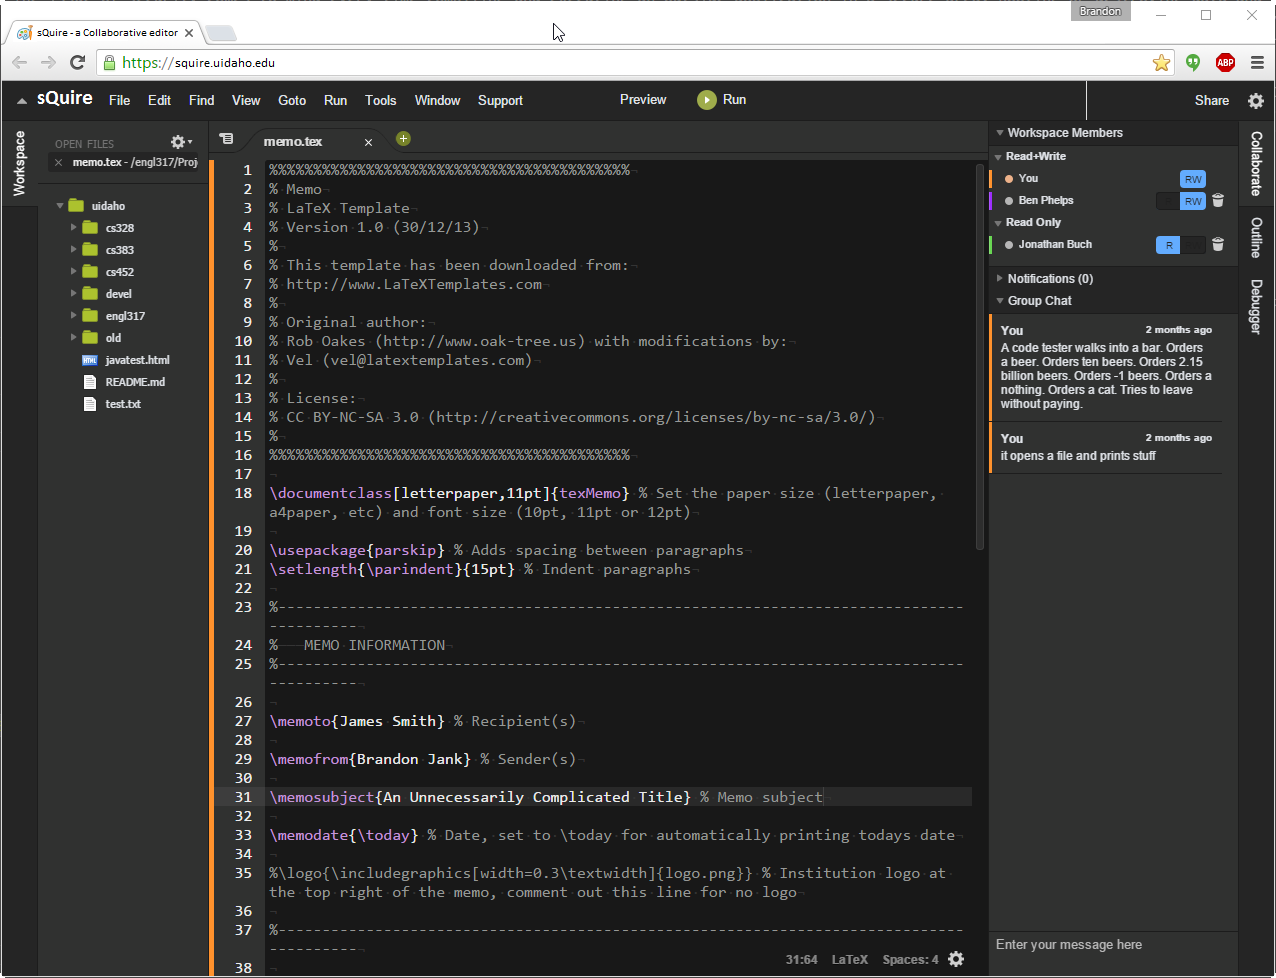
\includegraphics[width=0.7\textwidth]{mockups/mockup_squire_jank6275}
        \end{center}
        \captionof{figure}{"Squire is a web-based collaborative software development environment with a project development center. Squire will allow multiple users to edit files and communicate in real time. Projects can be ``stubbed'' out by a user and then other users can join and/or vote to support for their favorite projects. After a certain amount of support, planning, and documentation is reached for a project, the project becomes a fully fleged project and then community development can start. Think ``kickstarter for code'' where people pledge their help with the project and not just financial support."}
    \end{minipage}

\section{Core Features}
    \begin{itemize}
      \item Web based
      \item Some Common IDE features
      \item Collaborative tools
      \item Encapsulated Workspaces
      \item Compile and Download
      \item Self Destructing Rooms
    \end{itemize}
    The central idea behind sQuire is a somewhat akin to a code hostel. A collaborative editor which provides private, but shareable on demand spaces, with a low overhead for creation and ease of use. These spaces are meant for short term use, over an indeterminate period. Once the collaboration is done, the space is cleared and made available for others to use.
    
    With this vision in mind, sQuire best accomodates its users by being a browser based application. There should be no need for a user to download a client program, which would require periodic updates and ultimately require deletion on the users' end. By doing all of the collaboration and storage on a central server, accessed by the browser, we can make it more accessible to a wider audience. It may also encourage the development of collaborative "toy" projects by making it easier to start project spaces and find assistance when a project stalls.
    
    sQuire will be focused on coding in the Java language, though there are many worthwhile languages to choose from. Focusing on a single language will allow us to add more IDE-like features to assist in collaboration and make the language more accessible to those learning it.
    IDE-like Features:
    \begin{itemize}
      \item Key word color coding
      \item Parenthesis mismatch detection
      \item Missing end of line detection/prompting
    \end{itemize}
    
    sQuire is a collaborative tool, rather than a fully featured IDE with step through run-time debugging. Its features should be geared towards making it easier to debug code collaboratively, in the browser, without over-reliance on other tools. At a minimum, it needs:
    \begin{itemize}
      \item Native chat functionality
      \item Author attribution for code (colored underlining, footnote, etc.)
      \item Ability to "jump to" another user's cursor
      \item Ability to import/export code as plain text
      \item Account based access to projects
    \end{itemize}
    
    Collaborative features that would be "nice":
    \begin{itemize}
      \item Ability to save/restore to "snapshots" of the project
      \item Achievement and statistic tracking
    \end{itemize}
    
    User workspaces will be encapsulated, for both security and privacy. This could be accomplished using a container solution such as Docker or lmctfy (a free Google version). Containers have a lower performance hit to the host server than virtual machines, which are also a commonly implemented solution.  
    
    While security is a concern, we hope to address this using user space encapsulation, and by not running user code on the server. When users compile code, the compiled jar is downloaded and run locally from their own machines. While this means users are responsible for vetting the function of the code before running it on their machines, it means that our server resources are not being used as part of a bot net or similar exploit.
    
    Finally rooms must be self-destructing. For the convenience of the user, deletion of the space should be automatic after an appropriate period of inactivity. While a notification email should be sent to the space owner prior to deletion, again no user intervention should be required.

\section{Storage and Organization}
    The squire program will have a top down directory structure.
    Under the top domain, each individual registered user will have the ability to create projects (rooms) where they can build their program. 
    Inside the room the user will be able to create any number of files or pages to keep track of their project. 
    They will also have the ability to import and export files to and from their own machine and the project. 
    After creation the user will be able to switch between projects and create and delete pages from within the project itself.  
    They will have the ability to share their projects and invite other users to read or edit their work. 
    All of the user data, as well as each user’s relevant project and page information, as well as who has access to each project will be stored and maintained by a MySQL database.

\section{Execution}
    The Squire program will have a browser based client. Squire users can use this client to login their account, manipulate their project, and logout. The Squire editor will run clientside through Ace. Ace is an embeddable code editor written in JavaScript. It can be easily embedded in any web page, JavaScript application, and browser based client. On the other hand, the user data, user project, and edit information will saved in a MySQL database on the owner's hard drive.  

\section{Collaboration}
    The code editor will be a collaborative editor. Multiple users can edit the same file at the same time. This means that any changes one user makes need to be synced to the server, and then to the editors of any other users editing the same file. Some research shows that all popular collaborate editors (Google Docs, Cloud 9, etc) use an algorithm called Operational Transformation. On a basic level, this algorithm works by treating every change to a file as either an insert command, or a delete command. These commands are synced across clients to keep the file state the same. Squire will need something similar. It looks like there are several open source implementations of this algorithm, notably OT.js. These may or may not be adequate for use in Squire.
 
\section{Achievement System}
    In order to make Squire interesting, but still retain its usability, Squire will contain an achievement system. Achievements will be publicly visible to all users in the user's profile. When a user gains an achievement, it will be announced in the project chat. Achievements should be fun, and should be obtainable just by writing code (i.e, users shouldn’t have to actively try to get achievements). Some possible achievements: Lucky Break (a file compiles successfully on the first try), Social Butterfly (a user joins a project that has 10+ users), Job Security (Write a 1000+ line file without any comments).
    
\section{Chat System}
    We will most likely use a websocket-based chat system for sQuire, as it allows the easiest modification; Users and their coded colors will be listed, and their names next to their chat lines. The goal is to make a simple and lightweight, secure chat that allows users to collaborate with each other in an area outside the workspace.

\section{Permissions System (bolt1003)}
    Squire will have a permissions system that encompasses files, folders, users and rooms. The administrator will have the ability to delegate permission to other users.  The administrator will have the ability to set global permissions to users to control read, write, execute, room creation and sharing.  Each room with have its own set of permissions. These permissions are controlled by the moderator that is assigned to that room and the administrator. By default the creator of the room is the moderator of the room but this duty can be delegated to another if desired. The system has three default user groups, Administrator, Moderators and Users. Users have the ability to read, write and execute code by default. Moderators have the ability to manage rooms by adding or removing users to their rooms, creating sub-rooms and managing moderators for those rooms. Administrators have all encompassing power over all permissions in the system.

\section{Interface Structure (mora5651)}
    Since sQuire is an online collaborative editor, and interface structure plays a key roll in organizing all the features to fit properly. We decided in using Cloud9's interface as a base for sQuire's interface layout/structure. Cloud9 incorporates many of the same features as sQuire including file management, editor, and chat options. Other collaborative IDEs to consider Floobits, Kobra, and Codebox. 
    
\section{Security Nightmare (jank6275)}
    The issue of security comes to mind every time compiling and executing an outside application in a secure area. Rooting or destroying data and infrastructure is trivial when you are freely allowed to execute arbitrary Java. In order to allow for this functionality we must implement some type of security strategy. We could limit or block functionality in Java which is a cat and mouse game that breaks usability. We could compile and execute code on the client side. This would require a compiler written in JavaScript and cause compatibility issues on certain clients with reduced permissions or an exotic build environment. Or we could just Docker.


    Docker allows us to create containers that contain not only the user's build environment, but the server infrastructure to host their project. Containers include the application and all of its dependencies, but share the kernel with other containers. Simply put, users can destroy their own containers but nobody else’s. Obviously we will want to harden against known and obvious vectors, but at least any damage a user can do is limited to their own project. Containerization also allows us to take snapshots so that even if something goes wrong, we can always revert back to a working state.


%##########################################################################################################################################################################
% Requirements Documentation
%##########################################################################################################################################################################

\chapter{Requirements Documentation}
\section{Functional Requirements}
    Functional requirements will specify a behaviour or function. Squire's functional requirements are:
    \subsection{Authentication (mora5651)}
        \begin{itemize}
            \item Login to squire. (Usecase 4.1.2 and Class 5.2)
            \item Register for squire. (Usecase 4.1.1 and Class 5.2)
            \item Forgot username. (Usecase 4.1.4 and Class 5.2)
            \item Forgot password. (Usecase 4.1.5 and Class 5.2)
            \item Logout of squire. (Usecase 4.1.3 and Class 5.2)
        \end{itemize}
    \subsection{Project Management (bolt1003)}
        \begin{itemize}
            \item Create Project (Usecase 4.5.1 and Class 5.3)
            \item Open a project (Usecase 4.5.2 and Class 5.3)
            \item Join Project (Usecase 4.5.3 and Class 5.3)
            \item Leave project (Usecase 4.5.4 and Class 5.3)
            \item Delete Project (Usecase 4.5.5 and Class 5.3)
            \item Export Project (Usecase 4.5.6 and Class 5.3)
            \item Accept Invite to Project (Usecase 4.5.7 and Class 5.3)
            \item Remove User from Project (Usecase 4.5.8 and Class 5.3)
            \item Edit Project Permissions (Usecase 4.5.9 and Class 5.3)
            \item Invite User to Project (Usecase 4.5.10 and Class 5.3)
            \item Promote User to Admin (Usecase 4.5.11 and Class 5.3)
            \item Demote Admin (Usecase 4.5.12 and Class 5.3)
            \item Block User (Usecase 4.5.13 and Class 5.3)
        \end{itemize}
    \subsection{Project Ideas (mars2681)}
        \begin{itemize}
            \item Page to browse potential projects (Usecase 4.2 and Class 5.4)
            \item Up- and down-votes for project selection (Usecase 4.2 and Class 5.4)
            \item Different ways to sort projects (date, projected team size, votes) (Usecase 4.2 and Class 5.4)
            \item Ability to post a project (Usecase 4.2 and Class 5.4)
            \item Ability to edit a project (Usecase 4.2 and Class 5.4)
            \item Ability to delete a project (but only by project author) (Usecase 4.2 and Class 5.4)
            \item Ability to follow a project (Usecase 4.2 and Class 5.4)
        \end{itemize}
    \subsection{Settings - Preferences and Profile (brec9824)}
        \begin{itemize}
            \item Viewable profile by other users and by oneself (Usecase 4.6.1 and Class 5.5)
            \item Includes editable email, profile image, password, and personal bio. (Usecase 4.6.2 and Class 5.5)
            \item Setting for public, friends only, or private viewing of online status, email address, personal bio, project ownerships, project memberships, and friends list. (Usecase 4.6.3 and Class 5.5)
            \item Option for settings users prefered color and shape to be displayed in projects if available. (Usecase 4.6.2 and Class 5.5)
            \item Option to have account deleted. (Usecase 4.6.4 and Class 5.5)
        	\item Direct access to projects that are listed under project ownerships and project memberships. (Usecase 4.6.5 and Class 5.5)
        \end{itemize}
    \subsection{Compiler (boss2849)}
        \begin{itemize}
            \item Compile project sub-modules or entire project. (Usecase 4.7.1 and Class 5.6)
            \item Compile and run code within IDE. (Usecase 4.7.2 and Class 5.6)
            \item Compile code and package to a JAR. (Usecase 4.7.3 and Class 5.6)
            \item Impose temporary code freeze during compilation. (Usecase 4.7.4 and Class 5.6)
        \end{itemize}
    \subsection{Syntax (gall7417)}
        \begin{itemize}
            \item Parse lines of users code as it is written
            \item Color code various objects in the code such as variables and conditionals
            \item Report error feedback for any syntactical errors found
        \end{itemize}
    \subsection{Communication (jank6275)}
        \begin{itemize}
            \item Global chat when anywhere in program. (Usecase 4.3.2 and Class 5.8)
            \item Project chat when a project is open. (Usecase 4.3.1 and Class 5.8)
            \item Closeable project chat. (Usecase 4.3.3 and Class 5.8)
            \item Closeable global chat. (Usecase 4.3.4 and Class 5.8)
        \end{itemize}
   \subsection{Project File Editor (snev7821)}
        \begin{itemize}
            \item Add new file to project. (Usecase 4.4.1 and Class 5.9)
            \item Import existing file in to project. (Usecase 4.4.2 and Class 5.9)
            \item Delete a file. (Usecase 4.4.3 and Class 5.9)
            \item Export a file. (Usecase 4.4.4 and Class 5.9)
            \item Open file in new tab. (Usecase 4.4.5 and Class 5.9)
            \item View line numbers. (Usecase 4.4.6 and Class 5.9)
            \item View References. (Usecase 4.4.7 and Class 5.9)
            \item View Dates. (Usecase 4.4.8 and Class 5.9)
            \item View users and user history. (Usecase 4.4.9 and Class 5.9)
            \item Format Document. (Usecase 4.4.10 and Class 5.9)
            \item Find and replace. (Usecase 4.4.11 and Class 5.9)
            \item Display the currently typing user. (Usecase 4.4.12 and Class 5.9)
        \end{itemize}
    \subsection{Security (gall7417)}
        \begin{itemize}
            \item Resource defense strategy that includes not subjecting any sQuire server to becoming unresponsive due to a runaway program, and not allowing any sQuire server to give up shell access via an executing program in sQuire.
            \item Require authentication to access all user files and user information.
            \item Ensure confidentiality of all user information.
            \item Mitigate security threats by testing against common abuse cases and vulnerabilities.
            \item Ensure proper character sets for all input given.
            \item Enforce authorization controls on all system requests.
            \item Restrict access to resources and files outside of the users given resources.
        \end{itemize}

    
\section{Non-Functional Requirements}
    Non-functional requirements cover all the remaining requirements which are not covered by the functional requirements. They specify criteria that judge the operation of a system, rather than specific behaviours. Squire's non-functional requirements are:
    \begin{itemize}
        % Performance (jank6275)
        \item The current location of any user's cursor can be quickly jumped to by any user with the project open. (Usecase 4.5.8 and Class 5.9)
        \item Text written by the user in the editor should be visible instantaneously. (Usecase 4.5 and Class 5.9)
        \item Text written by other users in the editor should be visible within 2 seconds. (Usecase 4.5 and Class 5.9)
        \item Text will be underlined in the user's color, if they edited/created that text. (Usecase 4.5.9 and Class 5.9)
        \item The line number will be highlighted in the users color, if they created the line. (Usecase 4.5.9 and Class 5.9)
        \item Each line edited by a user should be saved to create a edit history for each user in a document. (Usecase 4.5.4 and Class 5.9)
        % Scalability (boss2849)
        \item The system should be designed in such a way that will easily and reliably scale to accommodate a growing user base. One method of dealing with scalability would be allowing the core system to reactively spawn new slaves to aid in computational needs, such as compilation. (boss2849)
        % Capacity (boss2849)
        \item Limited space for projects that haven't been initiated (enough for documentation, images, etc.) (boss2849)
        \item Reactively increasing capacity for projects proportional to the absolute needs of the projects. (no fluff) (boss2849)
        \item Encourage developers to store large files elsewhere, e.g. GitHub LFS, AWS, etc. (boss2849)
        % Availability (brec9824) 
        \item Since sQuire is web based, downtime for the servers most be kept to a minimum and be no more then once or twice a week for a few hours. This downtime will allow for database uprgrades and backups. (brec9824)
        % Reliability (bolt1003) 
        \item sQuire will leverage technology developed for the web to ensure reliablity. Technologies such as redunant hardware, redunant power providers, redunant internet services, load balancing and virtualization will enable sQuire to be reliable.(bolt1003)
        % Recoverability (mora5651) 
        \item SQuire will have the ability for the user to save on sQuire's database for recoverability isurance. It will also incorporate autosave feature. (mora5651)
        % Maintainability (mora5651) 
        \item Since sQuire is a web based application running on a webhost. There are 
        many maintenance tools that can be used to track performance. Maintainability of sQuire will also include regular backup schedules, speed test, and security monotoring. (mora5651)
        % Serviceability (bolt1003) 
        \item sQuire will run in a virtual machine on top of redunant hardware. Using a virtual machine allows for mutliple instance to be running and tested. The backend will run on redunant hardware which will prevent hardware failure from affecting sQuire usage. In turn, allowing infrastructure to be serviced without affecting sQuire. (bolt1003)
        % Security (jank6275)
        \item Each project should be containerized so that users can't harm each others projects. (jank6275)
        % Regulatory (mars2681) 
        \item Upon creation of account, user must agree to terms and conditions. (mars2681)
        \item User must comply with DMCA (Copy right law) (mars2681)
        \item User must confirm they are 18 or older (COPPA law) (mars2681)
        % Manageability (brec9824) 
        \item Will include monitoring of subsystems to collect and report performance data. (brec9824)
        \item Subsystem monititory must be highly efficient and take up less than 10\% of resources to keep noticeability to a minimum. (brec9824)
        \item Subsystems must be modular to allow for efficient monitoring, implementation of subsystems, and the addition of new subsystems. (brec9824)
        % Environmental (gall7417) 
        \item sQuire will run as a browser application in google chrome. (gall7417)
        \item sQire will run on virtually all modern processors. (gall7417)
        % Data Integrity (gall7417) 
        \item sQuire will use tcp to for reliable data communications. (gall7417)
        \item sQuire will use error checking upon large changes to ensure no drastic data corruption occurs. (gall7417)
        \item sQuire will use a history/autosave feature in case of data loss. (gall7417)
        % Usability (snev7821) 
        \item Provides code compilation and file system for users with limited resources. (snev7821)
        \item Easy to learn system, helpful syntax highlighting. (snev7821)
        \item More satisfying than competitors products, because of social/kickstarter aspect. (snev7821)
        % Interoperability (snev7821) 
        \item Provides github integration. (snev7821)
        \item Runs on any of the main browsers (chrome, firefox, safari). (snev7821)
        \item Due to web based design, works on lower end machines. (snev7821)
    \end{itemize}

%##########################################################################################################################################################################
% Use Case Diagrams
%##########################################################################################################################################################################

\chapter{Use Case Diagrams}
    \section{Overview (jank6275)}
        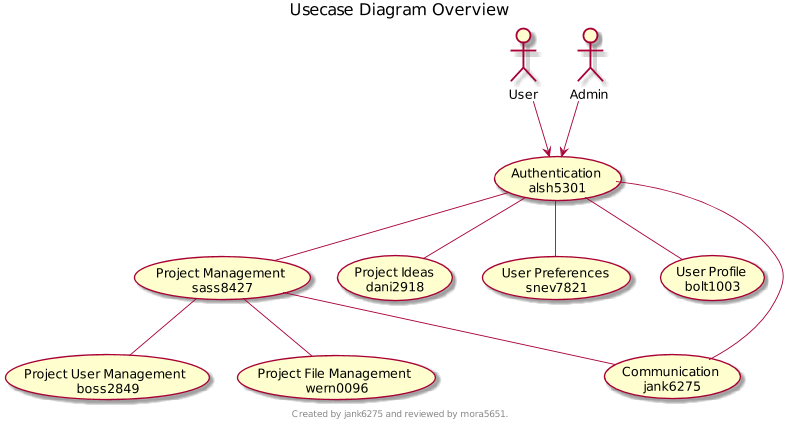
\includegraphics[width=\textwidth]{diagrams/usecase-overview}
        A usecase diagram that relates major sections of Squire.
    \section{Authentication (mora5651)}
        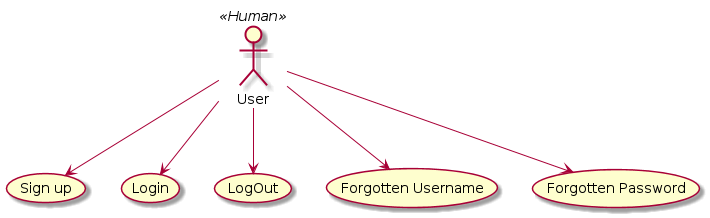
\includegraphics[width=\textwidth]{diagrams/usecase-authentication}
    \section{Project Ideas (mars2681)}
        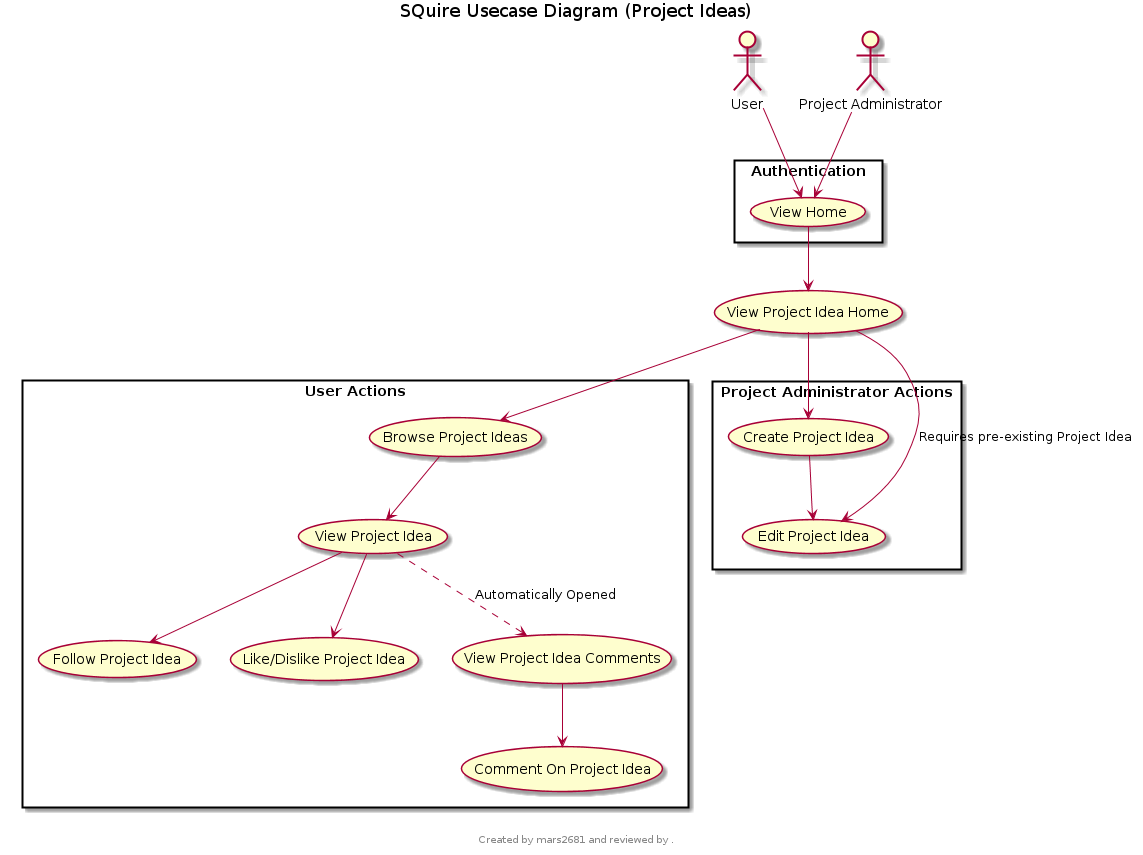
\includegraphics[width=\textwidth]{diagrams/usecase-projectideas}
    \section{Communication (jank6275)}
        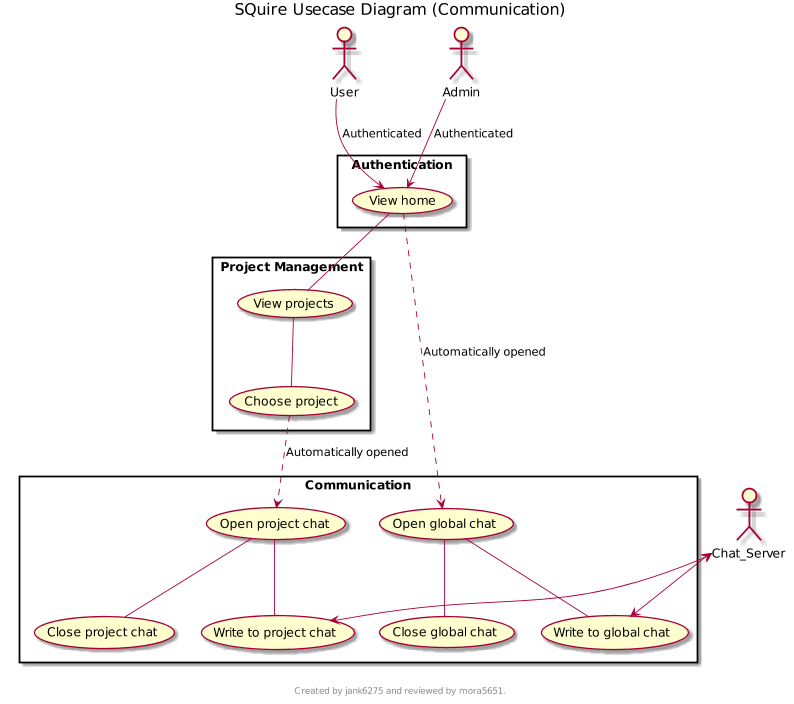
\includegraphics[width=\textwidth]{diagrams/usecase-communication}
        A usecase diagram for sQuire\'s communication features. Used in Class Diagrams 4.2.1 and 4.2.2.
    \section{User Preferences (snev7821)}
        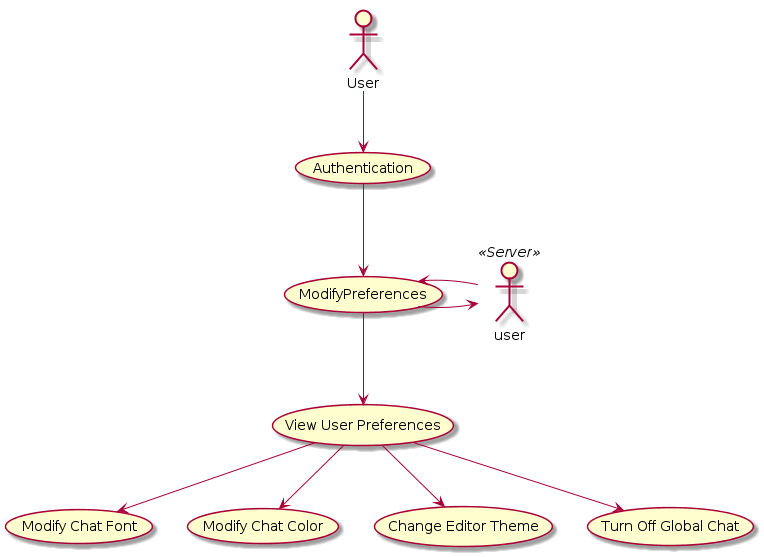
\includegraphics[width=\textwidth]{diagrams/usecase-preferences}
    \section{Project Management (bolt1003)}
        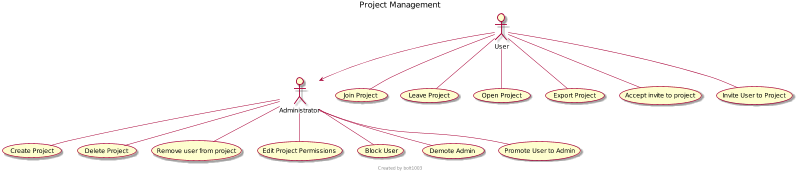
\includegraphics[width=\textwidth]{diagrams/usecase-projectmanagement}
    \section{Settings, Preferences, and Profile (brec9824)}
        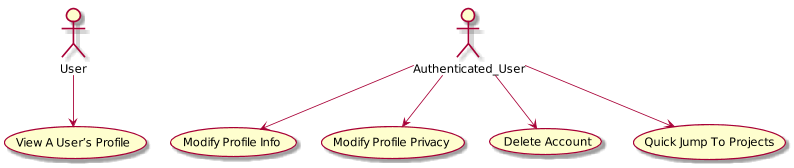
\includegraphics[width=\textwidth]{diagrams/usecase-settingsmanager}
    \section{Compiler (boss2849)}
        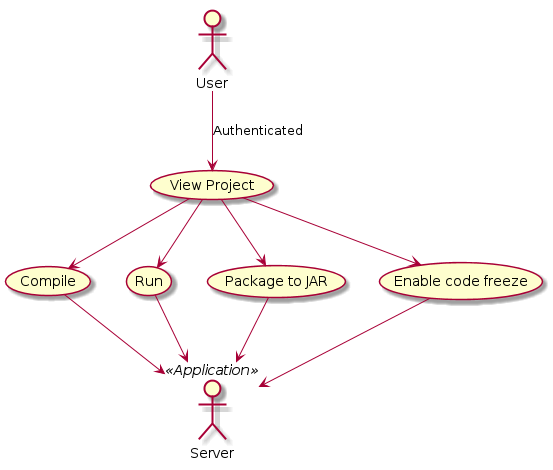
\includegraphics[width=\textwidth]{diagrams/usecase-compiler}
    
    
    
    

%##########################################################################################################################################################################
% Use Case Descriptions
%##########################################################################################################################################################################

%% TODO: ucd's still need rename, reorder and reformat -jank6275

\chapter{Use Case Descriptions}

\section{Authentication (mora5651)}
\subsection{Sign up (Use Case Diagram 3.2)}
    \begin{tabular}{ p{2cm} p{12cm} }
        \hline
        \\
        \textit{Actors:} & User. \\ 
        \\
        \textit{Goals:} & To register and create an account in sQuire. \\
        \\
        \textit{Pre-conditions:} & None. \\
        \\
        \textit{Summary:} & The user signs up and creates an account using their email address and, creates a username and password. \\ 
        \\
        \textit{Related use cases:} & Sign Up. \\ 
        \\
        \textit{Steps:} & \begin{enumerate}
            \item User is prompted to enter email, username and password. 
            \item System sends confirmation email. 
            \item User verifies email. 
            \item System saves information, and redirectes user to sign in page. 
        \end{enumerate} \\
        \\
        \textit{Alternative 1:} & User already has an account. \\ 
        \\
        \textit{Alternative 2:} & User doesn't confirm email. Delete request after timeout period. \\
        \\
        \hline
    \end{tabular}

\subsection{Sign in (Use Case Diagram 3.2)}
    \begin{tabular}{ p{2cm} p{12cm} }
        \hline
        \\
        \textit{Actors:} & Users. \\ 
        \\
        \textit{Goals:} & Pre-existing user signs into profile. \\
        \\
        \textit{Precondition:} & User must already have an account \\
        \\
        \textit{Summary:} & User wishes to access their account, projects and info. \\
        \\
        \textit{Related use cases:} & Comment on Project Idea \\ 
        \\
        \textit{Steps:} & \begin{enumerate}
            \item User is prompted to enter username/e-mail, and password. 
            \item System verifies information
            \item Correct information prompts user to their home page. 
        \end{enumerate} \\
        \\
        \textit{Alternatives:} & Information is incorrect, user tries again. Or makes a new account \\
        \\
        \hline
    \end{tabular}

\subsection{Logout (Use Case Diagram 3.2)}
\begin{tabular}{ p{2cm} p{12cm} }
 \hline
 \\
 \textit{Actors:} & Users. \\ 
  \\
 \textit{Goal:} & Existing user logs out \\ 
 \\
 \textit{Precondition:} & User must be logged in \\
 \\
 \textit{Summary:}  & The user can log-out of the program at any time. \\
 \\
 \textit{Steps:} & \begin{enumerate}
 \item User clicks the "log-out" button. 
 \item System prompts user to ensure all unsaved work has been saved. 
 \item User verifies. 
 \item System logs user out. 
 \end{enumerate} \\
\\
  \textit{Alternative 1:} & The program will send notification to ask if the user is sure to sign out. \\
  \textit{Alternative 2:} & User cancels on step two. Return to home page. \\ 
 \\
\hline
\end{tabular}

\subsection{Forgotten Username (Use Case Diagram 3.2)}
\begin{tabular}{ p{2cm} p{12cm} }
 \hline
 \\
 \textit{Actors:} & Users. \\ 
  \\
 \textit{Goal:} & Recover forgotten username. \\ 
 \\
 \textit{Precondition:} & User must already have an account. \\
 \\
 \textit{Summary:}  & User has forgotten their username, and wishes to recover it. \\
 \\
 \textit{Steps:} & \begin{enumerate}
    \item User clicks the "Forgotten username" button.
    \item User inputs their email address.
    \item System validates their email address with an account, and sends an email with the username.
 \end{enumerate} \\
\\
  \textit{Alternative 1:} & Information is incorrect, user tries again. Or makes a new account. \\
\\
\hline
\end{tabular}

\subsection{Forgotten Password (Use Case Diagram 3.2)}
\begin{tabular}{ p{2cm} p{12cm} }
 \hline
 \\
 \textit{Actors:} & Users. \\ 
  \\
 \textit{Goal:} & Recover forgotten password. \\ 
 \\
 \textit{Precondition:} & User must already have an account. \\
 \\
 \textit{Summary:}  & User has forgotten their password, and wishes to recover it. \\
 \\
 \textit{Steps:} & \begin{enumerate}
 \item User clicks the "Forgotten password" button. 
 \item User inputs their email address. 
 \item System validates their email address with an account. 
 \item System sends an email for the password reset. 
 \end{enumerate} \\
\\
  \textit{Alternative 1:} & Information is incorrect, user tries again. Or makes a new account. \\
\\
\hline
\end{tabular}

\section{Project Ideas (mars2681)}
\subsection{Browse Project Ideas }
\begin{tabular}{ p{2cm} p{12cm} }
 \hline
 \\
 \textit{Actors:} & User \\ 
 \\
 \textit{Goals:} & Browse new projects, popular projects, and user's projects\\
 \\
 \textit{Pre-conditions:} & User is signed in  \\
 \\
 \textit{Summary:} & User looks through posted project ideas to find projects to work on/discuss \\ 
 \\
 \textit{Related use cases:} & View Project Idea  \\ 
 \\
 \textit{Steps:} & \begin{enumerate}
  \item Actor selects Browse Project Ideas button, they are then brough to Project Ideas page
  \item System displays the project pages that the user is following, also the most popular projects, and new projects
 \end{enumerate} \\
 \\
 \textit{Alternatives:} & None. \\
 \\
 \textit{Post-conditions:} & None. \\
 \\
\hline
\end{tabular}

\subsection{View Project Idea}
\begin{tabular}{ p{2cm} p{12cm} }
 \hline
 \\
 \textit{Actors:} & User \\ 
 \\
 \textit{Goals:} & View project idea page  \\
 \\
 \textit{Pre-conditions:} & User is signed in and in the Browse Project Ideas page  \\
 \\
 \textit{Summary:} &  User views a project ideas page to look at its information and follow/comment/like or dislike. \\ 
 \\
 \textit{Related use cases:} & Browse Project Ideas\\ 
 \\
 \textit{Steps:} & \begin{enumerate}
  \item Actor selects a project from the Browse Project Ideas Page
  \item System brings actor to the project's info page
  \item Actor can then look at the projects information, as well as continue on to follow or comment or vote on the project idea

 \end{enumerate} \\
 \\
 \textit{Alternatives:} & None. \\
 \\
 \textit{Post-conditions:} & None. \\
 \\
\hline
\end{tabular}

\subsection{Create Project Idea}
\begin{tabular}{ p{2cm} p{12cm} }
 \hline
 \\
 \textit{Actors:} & Project Administrator \\ 
 \\
 \textit{Goals:} & Generate public interest in project idea  \\
 \\
 \textit{Pre-conditions:} & Prospective project administrator is signed in  \\
 \\
 \textit{Summary:} &  Admin can make a page to show off their project idea to other users \\ 
 \\
 \textit{Related use cases:} & Manage Project Idea Thread \\ 
 \\
 \textit{Steps:} & \begin{enumerate}
  \item Actor selects Create Project Idea button
  \item Actor enters prospective project title and thoughts and ideas as a description
  \item Actor selects Submit button
  \item System adds the project page to the database for other users to see

 \end{enumerate} \\
 \\
 \textit{Alternatives:} & None. \\
 \\
 \textit{Post-conditions:} & None. \\
 \\
\hline
\end{tabular}

\subsection{Edit Project Idea }
\begin{tabular}{ p{2cm} p{12cm} }
 \hline
 \\
 \textit{Actors:} & Project Administrator \\ 
 \\
 \textit{Goals:} & User edits the information on their project idea page \\
 \\
 \textit{Pre-conditions:} & Prospective project administrator is signed in and is now in the project idea page \\
 \\
 \textit{Summary:} &  User edits their pre-existing project idea page \\ 
 \\
 \textit{Related use cases:} & Create Project Idea Thread \\ 
 \\
 \textit{Steps:} & \begin{enumerate}
  \item Actor clicks Edit Project Idea Page
  \item Actor can then edit the title, description, and other information on the project idea page
  \item Actor clicks Submit
  \item System saves changes, updates page
  
 \end{enumerate} \\
 \\
 \textit{Alternatives:} & Actor selects Delete Changes and returns to Browse Project Ideas page. \\
 \\
 \textit{Post-conditions:} & None. \\
 \\
\hline
\end{tabular}

\subsection{Comment on Project Idea}
\begin{tabular}{ p{2cm} p{12cm} }
 \hline
 \\
 \textit{Actors:} & User \\ 
 \\
 \textit{Goals:} & Provide detailed feedback on project ideas  \\
 \\
 \textit{Pre-conditions:} & Actor is signed in, has navigated to a project idea  \\
 \\
 \textit{Summary:} &  User provides feedback to or asks questions about a prospective project. \\ 
 \\
 \textit{Related use cases:} & Browse Project Ideas, Vote on Project Idea, Manage Project Idea Thread \\ 
 \\
 \textit{Steps:} & \begin{enumerate}
  \item Actor selects Comment button
  \item Actor types feedback into field 
  \item Actor clicks Submit button
  \item System shows confirmation that feedback was received 
  \item System adds comment to Project Idea page's comments
 \end{enumerate} \\
 \\
 \textit{Alternatives:} & None \\
 \\
 \textit{Post-conditions:} & None. \\
 \\
\hline 
\end{tabular}

\subsection{Like/Dislike Project Idea}
\begin{tabular}{ p{2cm} p{12cm} }
 \hline
 \\
 \textit{Actors:} & User \\ 
 \\
 \textit{Goals:} & Support promising project ideas or offer criticism to unfavorable ones  \\
 \\
 \textit{Pre-conditions:} & Actor is signed in, has navigated to a project idea  \\
 \\
 \textit{Summary:} &  User offers support/discourages a project idea so that prospective project administrators get feedback and promising project ideas get publicity \\ 
 \\
 \textit{Related use cases:} & Comment on Project Idea \\ 
 \\
 \textit{Steps:} & \begin{enumerate}
  \item Actor selects and Up Vote or Down Vote button
  \item Actor selects Submit button 
  \item System highlights which button the user has selected
 \end{enumerate} \\
 \\
 \textit{Alternatives:} & None \\
 \\
 \textit{Post-conditions:} & None. \\
 \\
\hline
\end{tabular}

\subsection{Follow Project Idea}
\begin{tabular}{ p{2cm} p{12cm} }
 \hline
 \\
 \textit{Actors:} & User, Project Administrator \\ 
 \\
 \textit{Goals:} & Follow project updates  \\
 \\
 \textit{Pre-conditions:} & Actor is signed in, has navigated to a project idea  \\
 \\
 \textit{Summary:} &  User follows project to receive updates and information about it \\ 
 \\
 \textit{Related use cases:} & View Project Idea \\ 
 \\
 \textit{Steps:} & \begin{enumerate}
  \item Actor selects Follow button
  \item System notifies user that they are now following the project
  \item System automatically updates followed project information on Browse Project Ideas page
 \end{enumerate} \\
 \\
 \textit{Alternatives:} & None \\
 \\
 \textit{Post-conditions:} & None. \\
 \\
\hline
\end{tabular}



\section{Communication (jank6275)}
\subsection{Open project chat (Class Diagram 5.8)}
\begin{tabular}{ p{2cm} p{12cm} }
 \hline
 \\
 \textit{Actors:} & User \\ 
 \\
 \textit{Goals:} & To open the project chat window. \\
 \\
 \textit{Pre-conditions:} & User must be registered, signed in, and have a open project.  \\
 \\
 \textit{Summary:} & User opens a project and the project chat automatically opens. The chat window displays chat history and updates when new chat messages are received. \\ 
 \\
 \textit{Related use cases:} & Join global chat. \\ 
 \\
 \textit{Steps:} & \begin{enumerate}
  \item User opens a project.
  \item Chat is notified that user has joined.
  \item System displays project chat window to the user.
 \end{enumerate} \\
 \\
 \textit{Alternatives:} & None. \\
 \\
 \textit{Post-conditions:} & None. \\
 \\
\hline
\end{tabular}

\subsection{Open global chat (Class Diagram 5.8)}
\begin{tabular}{ p{2cm} p{12cm} }
 \hline
 \\
 \textit{Actors:} & User \\ 
 \\
 \textit{Goals:} & To open the global chat window. \\
 \\
 \textit{Pre-conditions:} & User must be registered, signed in, and anywhere on website.  \\
 \\
 \textit{Summary:} & User authenticates with the server and the global chat automatically opens. The chat window displays chat history and updates when new chat messages are received.  \\ 
 \\
 \textit{Related use cases:} & Join project chat. \\ 
 \\
 \textit{Steps:} & \begin{enumerate}
  \item User clicks open global chat.
  \item Chat is notified that user has joined.
  \item System displays global chat window.
 \end{enumerate} \\
 \\
 \textit{Alternatives:} & None. \\
 \\
 \textit{Post-conditions:} & None. \\
 \\
\hline
\end{tabular}

\subsection{Close project chat (Class Diagram 5.8)}
\begin{tabular}{ p{2cm} p{12cm} }
 \hline
 \\
 \textit{Actors:} & User \\ 
 \\
 \textit{Goals:} & To close the project chat window. \\
 \\
 \textit{Pre-conditions:} & User must be registered, signed in, and in editor Mode.  \\
 \\
 \textit{Summary:} & User clicks on close project chat and the chat window closes. \\ 
 \\
 \textit{Related use cases:} & Close global chat. \\ 
 \\
 \textit{Steps:} & \begin{enumerate}
  \item User clicks close project chat.
  \item Chat is notified that user has left.
  \item Client closes project chat window.
 \end{enumerate} \\
 \\
 \textit{Alternatives:} & None. \\
 \\
 \textit{Post-conditions:} & None. \\
 \\
\hline
\end{tabular}

\subsection{Close global chat (Class Diagram 5.8)}
\begin{tabular}{ p{2cm} p{12cm} }
 \hline
 \\
 \textit{Actors:} & User \\ 
 \\
 \textit{Goals:} & To close the global chat window. \\
 \\
 \textit{Pre-conditions:} & User must be registered, signed in, and anywhere on website.  \\
 \\
 \textit{Summary:} & User clicks on open global chat and the chat opens, displaying chat history and updating when needed. \\ 
 \\
 \textit{Related use cases:} & Close project chat. \\ 
 \\
 \textit{Steps:} & \begin{enumerate}
  \item User clicks close global chat.
  \item Chat is notified that user has left.
  \item Client closes global chat window.
 \end{enumerate} \\
 \\
 \textit{Alternatives:} & None. \\
 \\
 \textit{Post-conditions:} & None. \\
 \\
\hline
\end{tabular}

\subsection{Write to project chat (Class Diagram 5.8)}
\begin{tabular}{ p{2cm} p{12cm} }
 \hline
 \\
 \textit{Actors:} & User \\ 
 \\
 \textit{Goals:} & To send text to project chat. \\
 \\
 \textit{Pre-conditions:} & User must be registered, signed in, a project opened, with the project chat window open, and the text box selected.  \\
 \\
 \textit{Summary:} & User clicks in the project chat text box and then types a message then either presses enter or clicks the submit button. The text is displayed to all users in the chat, including the user. \\ 
 \\
 \textit{Related use cases:} & Write to global chat. \\ 
 \\
 \textit{Steps:} & \begin{enumerate}
  \item User clicks in the project chat box.
  \item User types a message and then presses enter or clicks submit button.
  \item Message is relayed to all clients with project chat open.
  \item Message is displayed.
 \end{enumerate} \\
 \\
 \textit{Alternatives:} & None. \\
 \\
 \textit{Post-conditions:} & None. \\
 \\
\hline
\end{tabular}

\subsection{Write to global chat (Class Diagram 5.8)}
\begin{tabular}{ p{2cm} p{12cm} }
 \hline
 \\
 \textit{Actors:} & User \\ 
 \\
 \textit{Goals:} & To send text to global chat. \\
 \\
 \textit{Pre-conditions:} & User must be registered, signed in, anywhere on website, with the global chat window open, and the text box selected.  \\
 \\
 \textit{Summary:} & User clicks in the global chat text box and then types a message then either presses enter or clicks the submit button. The text is displayed to all users in the chat, including the user. \\ 
 \\
 \textit{Related use cases:} & Write to project chat. \\ 
 \\
 \textit{Steps:} & \begin{enumerate}
  \item User clicks in the global chat box.
  \item User types a message and then presses enter or clicks submit button.
  \item Message is relayed to all clients with global chat open.
  \item Message is displayed.
 \end{enumerate} \\
 \\
 \textit{Alternatives:} & None. \\
 \\
 \textit{Post-conditions:} & None. \\
 \\
\hline
\end{tabular}

\subsection{Modify chat font (Settings Class Diagram)}
\begin{tabular}{ p{2cm} p{12cm} }
 \hline
 \\
 \textit{Actors:} & User \\ 
 \\
 \textit{Goals:} & To change a users font style inside the global and project chat. \\
 \\
 \textit{Pre-conditions:} & User must be registered, signed in, the user settings window opened, and the chat settings tab open.  \\
 \\
 \textit{Summary:} & The user clicks the settings menu and changes their font style for both the project and global chat through a drop down box of available fonts. \\ 
 \\
 \textit{Related use cases:} & Modify chat color. \\ 
 \\
 \textit{Steps:} & \begin{enumerate}
  \item User clicks the settings menu.
  \item User clicks chat settings tab.
  \item User clicks chat font drop down box.
  \item User clicks desired font.
  \item User clicks save.
  \item The user's selection is saved in the database.
  \item All further chat messages will use the selected font.
 \end{enumerate} \\
 \\
 \textit{Alternatives:} & None. \\
 \\
 \textit{Post-conditions:} & None. \\
 \\
\hline
\end{tabular}

\subsection{Modify chat color (Settings Class Diagram)}
\begin{tabular}{ p{2cm} p{12cm} }
 \hline
 \\
 \textit{Actors:} & User \\ 
 \\
 \textit{Goals:} & To change a users font color inside the global and project chat. \\
 \\
 \textit{Pre-conditions:} & User must be registered, signed in, the user settings window opened, and the chat settings tab open.  \\
 \\
 \textit{Summary:} & The user clicks the settings menu and changes their font color for both the project and global chat through a drop down box of available colors. \\ 
 \\
 \textit{Related use cases:} & Modify chat font. \\ 
 \\
 \textit{Steps:} & \begin{enumerate}
  \item User clicks the settings menu.
  \item User clicks chat settings tab.
  \item User clicks chat color drop down box.
  \item User clicks desired color.
  \item User clicks save.
  \item The user's selection is saved in the database.
  \item All further chat messages from the user will use the selected color.
 \end{enumerate} \\
 \\
 \textit{Alternatives:} & None. \\
 \\
 \textit{Post-conditions:} & None. \\
 \\
\hline
\end{tabular}

\section{Project File Editor (snev7821)}
\subsection{Add New File to Project}
\begin{tabular}{ p{2cm} p{12cm} }
\hline 
\\
 \textit{Actors:} & User of sQuire \\
 \\
 \textit{Summary:} & The user performs this task to add a new file to the project. \\
 \\
 \textit{Pre-conditions:} & \begin{enumerate}
  \item User must be registered.
  \item User must be logged in.
  \item User must have a project open.
 \end{enumerate} \\
 \\
 \textit{Steps:} & \begin{enumerate}
  \item User clicks File in the top menu bar.
  \item System opens a drop-down menu.
  \item User navigates to Add New File.
  \item System opens an Add New File dialog window.
  \item User selects the file type and names the file.
  \item User clicks Add.
  \item System adds the file to the project.
 \end{enumerate} \\
 \\
 \textit{Alternatives:} & \begin{enumerate}
  \item Step 1: The user right clicks in the project panel and the system continues on to step 2 above.
  \item Step 5: The user clicks Cancel and a new file is not added to the project.
 \end{enumerate} \\
 \\ 
 \textit{Post-conditions:} & \begin{enumerate}
  \item A new file is added to the project.
  \item The database is updated to reflect the changes.
 \end{enumerate} \\
 \\
 \textit{Related:} & Add Existing File to Project \\
 \\
\hline
\end{tabular} 
\newpage

\subsection{Add Existing File to Project}
\begin{tabular}{ p{2cm} p{12cm} }
\hline
 \\
 \textit{Actors:} & User of sQuire \\
	\\
	\textit{Summary:} & The user performs this task to add an existing file to the project. \\ 
	\\
	\textit{Pre-conditions:} & \begin{enumerate}
		\item User must be registered.
		\item User must be logged in.
		\item User must have a project open.
	\end{enumerate} \\
	\textit{Steps:} & \begin{enumerate}
		\item User clicks File in the top menu bar.
		\item System opens a drop-down menu.
		\item User navigates to Add Existing File.
		\item System opens an Add Existing File dialog window.
		\item User selects PC or SQuire or Github.
		\item System updates the dialog to reflect the selected source.
		\item User navigates to the file's location and selects it.
		\item User clicks Add.
		\item System adds the file to the project.
	\end{enumerate} \\
	\\
	\textit{Alternatives:} & \begin{enumerate}
		\item Step 1: The user right clicks in the project panel and the system continues on to step 2 above.
		\item Step 5-7: The user clicks Cancel and a new file is not added to the project.
	\end{enumerate} \\
	\\
	\textit{Post-conditions:} & \begin{enumerate}
		\item An existing file is added to the project.
		\item The database is updated to reflect the changes.
	\end{enumerate} \\
	\\
	\textit{Related:} & Add New File to Project \\
	\\
	\hline
\end{tabular}
\newpage

\subsection{Delete File}
\begin{tabular}{ p{2cm} p{12cm} }
\hline \\
	\textit{Actors:} & User of sQuire \\
	\\
	\textit{Summary:} & The user performs this task to delete a file from the project. \\
	\\
	\textit{Pre-conditions:} & \begin{enumerate}
		\item User must be registered.
		\item User must be logged in.
		\item User must have a project open.
		\item User must be administrator of project.
		\item Current project must have at least one file.
	\end{enumerate} \\
	\\
	\textit{Steps:} & \begin{enumerate}
		\item User right clicks a file in the project pane.
		\item System opens a drop-down menu.
		\item User navigates to \textit{Delete}.
		\item System opens an \textit{Delete File} dialog window, asking if the user is sure.
		\item User selects \textit{Yes}.
		\item System deletes the file from the project.
	\end{enumerate} \\
	\\
	\textit{Alternatives:} & \begin{enumerate}
		\item Step 5: The user clicks \textit{Cancel} instead and the file is not deleted from the project.
		\item The user selects multiple files before step 1.
	\end{enumerate} \\
	\\
	\textit{Post-conditions:} & \begin{enumerate}
		\item The file is deleted from the project.
		\item The database is updated to reflect the changes.
	\end{enumerate} \\
	\\
	\textit{Related:} & Delete Project \\
	\\
\hline
\end{tabular} 
\newpage


\subsection{Export Files}
\begin{tabular}{ p{2cm} p{12cm} }
\hline
	\\
	\textit{Actors:} & User of sQuire \\
	\\
	\textit{Summary:} & The user performs this task to download a number of files from a project. \\
	\\
	\textit{Pre-conditions:} &  \begin{enumerate}
		\item User must be registered.
		\item User must be logged in.
		\item User must have a project open.
		\item Must have at least one file in the project.
		\item User must have download permissions.
	\end{enumerate} \\
	\\
	\textit{Steps:} & \begin{enumerate}
		\item User clicks File in the top menu bar.
		\item System opens a drop-down menu.
		\item User navigates to Export Files.
		\item System opens an Export dialog window showing the project files on the left panel and the export location in the right panel.
		\item User selects a number of files on the left pane.
		\item User navigates to the export location in the right pane.
		\item User clicks Export.
		\item System downloads the selected files to the specified location.
	\end{enumerate} \\
	\\
	\textit{Alternatives:} & \begin{enumerate}
		\item Step 1: The user right clicks in the project panel and the system continues on to step 2 above.
		\item Step 5: User selects a folder and all files under that folder are selected.
		\item Step 5-6: The user clicks Cancel and the project is not exported.
	\end{enumerate} \\
	\\
	\textit{Related:} & Export Project \\
	\\
\hline
\end{tabular}
\newpage


\subsection{Open File in New Tab}
\begin{tabular}{ p{2cm} p{12cm} }
\hline
	\\
	\textit{Actors:} & User of sQuire \\
	\\
	\textit{Summary:} & Allows users to open a file. \\
	\\
	\textit{Goals:} & Opening files is essential in being able to work on a project. \\
	\\
	\textit{Pre-conditions:} &  \begin{enumerate}
		\item User is registered.
		\item User is logged in.
		\item User has a project open.
		\item Current project contains at least one file.
		\item User has read permission.
	\end{enumerate} \\
	\\
	\textit{Steps:} & \begin{enumerate}
		\item User double clicks a file.
		\item The editor opens its contents in a new tab and focuses on it.
	\end{enumerate} \\
	\\
	\textit{Alternatives:} & Step 1: Instead of double clicking a file, the user right clicks it and navigates to Open. \\
	\\
\hline
\end{tabular}
\newpage

\subsection{View Line Numbers }
\begin{tabular}{ p{2cm} p{12cm} }
\hline
\\
	\textit{Actors:} & User of sQuire \\
	\\
	\textit{Summary:} & Allows the user to hide line numbers to the left of the document. \\
	\\
	\textit{Goals:} & In case user wants to hide line numbers so they have more space for text.\\
	\\
	\textit{Pre-conditions:} & \begin{enumerate}
		\item Must be registered.
		\item Must be logged in.
		\item User has view permission.
		\item A file is open.
		\item Line numbers are on
	\end{enumerate} \\
	\\
	\textit{Steps:} & \begin{enumerate}
		\item User selects the View menu option.
		\item System displays a drop-down with various options.
		\item User selects the Hide Line Numbers option.
		\item System hides line numbers to the left of the document.
	\end{enumerate} \\
	\\
	\textit{Related:} & \begin{enumerate}
		\item View References
		\item View Dates
		\item View Authors
	\end{enumerate} \\
	\\
\hline
\end{tabular}
\newpage


\subsection{View References}
\begin{tabular}{ p{2cm} p{12cm} }
\hline
\\
	\textit{Actors:} & User of sQuire \\
	\\
	\textit{Summary:} & Allows the user to view the number of references to a given function. \\
	\\
	\textit{Goals:} & It is useful to know the number of references to a given function for optimization and debugging purposes. \\
	\\
	\textit{Pre-conditions:} &  \begin{enumerate}
		\item Must be registered.
		\item Must be logged in.
		\item User has view permission.
		\item A \textit{code} file is open.
	\end{enumerate} \\
	\\
	\textit{Steps:} & \begin{enumerate}
		\item User selects the View menu option.
		\item System displays a drop-down with various options.
		\item User selects the View References option.
		\item System displays the number of references above each method declaration.
	\end{enumerate} \\
	\\
	\textit{Related:} & \begin{enumerate}
		\item Hide Line Numbers
		\item View Dates
		\item View Authors
	\end{enumerate} \\
	\\
\hline
\end{tabular}
\newpage


\subsection{View Dates}
\begin{tabular}{ p{2cm} p{12cm} }
\hline \\
	\textit{Actors:} & User of sQuire \\
	\\
	\textit{Summary:} & Allows the user to view the last date that each block of a document was edited. Blocks are defined as any number of lines that was written by a single user. Minimum block size is one line. \\
	\\
	\textit{Goals:} & This provides a useful metric for how up-to-date parts of the document are. \\
	\\
	\textit{Pre-conditions:} & \begin{enumerate}
		\item Must be registered.
		\item Must be logged in.
		\item User has view permission.
		\item A file is open.
	\end{enumerate} \\
	\\
	\textit{Steps:} & \begin{enumerate}
		\item User selects the View menu option.
		\item System displays a drop-down with various options.
		\item User selects the View Dates option.
		\item System displays the last date that each block of a document was edited.
	\end{enumerate} \\
	\\
	\textit{Related:} & \begin{enumerate}
		\item Hide Line Numbers
		\item View References
		\item View Authors
	\end{enumerate} \\
	\\
\hline
\end{tabular}
\newpage


\subsection{View Authors}
\begin{tabular}{ p{2cm} p{12cm} }
\hline
\\
	\textit{Actors:} & User of sQuire \\
	\\
	\textit{Summary:} & Allows the user to view the last author that edited each block of a document. Blocks are defined as any number of lines that was written by a single user. Minimum block size is one line. \\
	\\
	\textit{Goals:} & This is an accountability tool allowing other users to identify who is responsible for a change to a document. \\
	\\
	\textit{Pre-conditions:} & 
	\begin{enumerate}
		\item Must be registered.
		\item Must be logged in.
		\item User has read permission.
		\item A file is open.
	\end{enumerate} \\
	\\
	\textit{Steps:} & \begin{enumerate}
		\item User selects the View menu option.
		\item System displays a drop-down with various options.
		\item User selects the View Authors option.
		\item System displays the name of the last editor of each line of the document.
	\end{enumerate} \\
	\\
	\textit{Related:} & \begin{enumerate}
		\item Hide Line Numbers
		\item View References
		\item View Dates
	\end{enumerate} \\
	\\
\hline
\end{tabular}
\newpage


\subsection{Format Document}
\begin{tabular}{ p{2cm} p{12cm} }
\hline \\
	\textit{Actors:} & User of sQuire \\
	\\
	\textit{Summary:} & Allows the user to format the document to a specified format \\
	\\
	\textit{Goals:} & An easy tool for making sweeping changes to a large part of a document. \\
	\\
	\textit{Pre-conditions:} & \begin{enumerate}
		\item Must be registered.
		\item Must be logged in.
		\item User has read/write permission.
		\item A file is open.
		\item The document has formatting options set.
	\end{enumerate} \\
	\\
	\textit{Steps:} & \begin{enumerate}
		\item User selects the Edit menu option.
		\item System displays a drop-down with various options.
		\item User selects the Format Document option.
		\item System formats the current document to the formatting settings currently set.
	\end{enumerate} \\
	\\
	\textit{Alternatives:} & \begin{enumerate}
		\item If no formatting settings are currently set, display a dialog box after step 3 and give the option for the user to do so now.
	\end{enumerate} \\
	\\
	\textit{Related:} & \begin{enumerate}
		\item Find/Replace
	\end{enumerate} \\
	\\
\hline
\end{tabular}
\newpage


\subsection{Find/Replace}
\begin{tabular}{ p{2cm} p{12cm} }
\hline
\\
	\textit{Actors:} & User of sQuire \\
	\\
	\textit{Summary:} &  Allows the user to find and/or replace phrases. \\
	\\
	\textit{Goals:} & This is a powerful tool that allows a user to make safer, quicker, and more efficient changes to a document. \\
	\\
	\textit{Pre-conditions:} &  \begin{enumerate}
		\item Must be registered.
		\item Must be logged in.
		\item User has read/write permission.
		\item A file is open.
	\end{enumerate}\\
	\\
	\textit{Steps:} & \begin{enumerate}
		\item User selects the Edit menu option.
		\item System displays a drop-down with various options.
		\item User selects the Find/Replace option.
		\item System displays a small form in an unobtrusive location.
		\item User enter the phrase to find and selects find.
		\item System highlights and focuses on the first occurrence of the phrase and all highlights all other occurrences.
	\end{enumerate} \\
	\\
	\textit{Alternatives:} & \begin{enumerate}
		\item User selects option to replace in step 5 and enters a phrase with which to replace the found occurrences of the searched phrase. The system replaces each occurrence.
	\end{enumerate} \\
	\\
	\textit{Related:} & \begin{enumerate}
		\item Format Document
		\item Find/Replace
	\end{enumerate} \\
	\\
\hline
\end{tabular}
\newpage

\subsection{Display Typing User}
\begin{tabular}{ p{2cm} p{12cm} }
\hline \\
	\textit{Actors:} & User of sQuire \\
	\\
	\textit{Summary:} & As the user types, the system displays their name, their typing, and their caret, in a different color, to other users. \\
	\\
	\textit{Goals:} & Differentiate who is typing what. \\
	\\
	\textit{Pre-conditions:} & \begin{enumerate}
		\item Must be registered.
		\item Must be logged in.
		\item User has read/write permission.
		\item A file is open.
		\item Other users have the same document open.
	\end{enumerate} \\
	\\
	\textit{Steps:} & \begin{enumerate}
		\item User begins typing.
		\item System displays the user's typing, the user's name, and the user's caret, in a different color, to Other Users.
		\item Other Users see User typing, his username, and his caret, in a different color.
	\end{enumerate} \\
	\\
\hline
\end{tabular}
\newpage

\section{Project Management (bolt1003) (Use Case Diagram: 3.6)}
\subsection{Create Project (Use Case Diagram: 3.6)}
\begin{tabular}{ p{2cm} p{12cm} }
 \hline
 \\
 \textit{Actors:} & Users of sQuire. \\ 
 \\
 \textit{Goals:} & Create a Project. \\
 \\
 \textit{Pre-conditions:} & The user is logged in and at the dashboard. \\
 \\
 \textit{Summary:} & The user creates a project. \\ 
 \\
 \textit{Related use cases:} & None. \\ 
 \\
 \textit{Steps:} & \begin{enumerate}
  \item User selects the "+" icon and a wizard appears.
  \item A name is choosen for the project.
  \item Language is selected from a drop down menu.
  \item User clicks finish.
 \end{enumerate} \\
 \\
 \textit{Alternatives:} & Create project from the editor. \\
 \\
 \textit{Post-conditions:} & The user assigns permissions to access the project. \\
 \\
\hline
\end{tabular}

\subsection{Open a project (Use Case Diagram: 3.6)}
\begin{tabular}{ p{2cm} p{12cm} }
 \hline
 \\
 \textit{Actors:} & Users of sQuire. \\ 
 \\
 \textit{Goals:} & Choose the desired project and open it. \\
 \\
 \textit{Pre-conditions:} & One or more projects are available, the user is logged in and at the dashboard. \\
 \\
 \textit{Summary:} & User looks through a list of projects and selects the desired project. \\ 
 \\
 \textit{Related use cases:} & None. \\ 
 \\
 \textit{Steps:} & \begin{enumerate}
  \item User clicks on projects in the menu bar.
  \item A list of projects appears and the user clicks on the desired project.
 \end{enumerate} \\
 \\
 \textit{Alternatives:} & Open a project from recent projects. \\
 \\
 \textit{Post-conditions:} & User closes sQuire. \\
 \\
\hline
\end{tabular}

\subsection{Join Project (Use Case Diagram: 3.6)}
\begin{tabular}{ p{2cm} p{12cm} }
\hline
\\
\textit{Actors:} & Users of sQuire. \\ 
\\
\textit{Goals:} & Join an existing project.\\
\\
\textit{Pre-conditions:} & Must be registered, logged in and have permission to join a project.\\
\\
\textit{Summary:} & The user logs in, chooses a project, and joins the project. \\
\\
\textit{Related use cases:} & Invite user to project, Accept user invite. \\
\\
\textit{Steps:} & \begin{enumerate}
 \item The user selects a project.
 \item The user chooses the "Join". 
 \item The project is added to the users projects bar.
 \item The user selects the project and selects "open".
\end{enumerate}\\
\\
\textit{Alternatives:} & User may decline an inventation to join a project. \\
\\
\textit{Post-conditions:} & None \\
\\
\hline
\end{tabular}

\subsection{Leave project (Use Case Diagram: 3.6)}
\begin{tabular}{ p{2cm} p{12cm} }
 \hline
 \\
 \textit{Actors:} & User \\ 
 \\
 \textit{Goals:} & Remove member status from project. \\
 \\
 \textit{Pre-conditions:} & Logged in, member of the respective project, not project owner.  \\
\\
 \textit{Summary:} & A member of a project can unjoin that project at any time as long as they are not the project owner. To prevent mistakenly unjoining a project, the user is asked to confirm their decision.\\ 
 \\
 \textit{Related use cases:} & \\ 
 \\
 \textit{Steps:} & \begin{enumerate}
  \item User selects a project.
  \item User clicks "Unjoin". 
  \item User is promted to confirm their decision
  \item User clicks "Confirm".
  \item User is removed from project member list.    
 \end{enumerate} \\
 \\
 \textit{Alternatives:} & User clicks "Cancel" at step 4, in which case the task is ends at that point. \\
 \\
 \textit{Post-conditions:} & None. \\
 \\
\hline
\end{tabular}

\subsection{Delete Project (Use Case Diagram: 3.6)}
\begin{tabular}{ p{2cm} p{12cm} }
\hline
\\
\textit{Actors:} & Users of sQuire.\\
\\
\textit{Goals:} & Delete an existing project. \\
\\
\textit{Pre-conditions:} & The user has the appropriate permissions to delete project. 
\\
\textit{Summary:} & A user deletes a project from the project workspace.\\
\\
\textit{Related use cases:} & Create a project. \\
\\
\textit{Steps:} & \begin{enumerate}
 \item The user selects a project.
 \item The user clicks on the "Delete project" button. 
 \item A dialog is displayed. 
 \item User select "delete" to delete the project. 
 \end{enumerate}\\
 \\
 \textit{Alternatives:} & User may choose not to delete the project in the confirmation display.\\
 \\
 \textit{Post-conditions:} & None. \\
 \\
\hline
\end{tabular}

\subsection{Export Project (Use Case Diagram: 3.6)}
\begin{tabular}{ p{2cm} p{12cm} }
\hline
\\
\textit{Actors:} & User of sQuire.\\
\\
\textit{Goals:} & Export a workspace to a local file. \\
\\
\textit{Pre-conditions:} & The user needs permission to export the project. 
\\
\textit{Summary:} & User saves a file containing the project settings and files to a local machine. \\
\\
\textit{Related use cases:} & Importing a project, Creating a new project. \\
\\
\textit{Steps:} & \begin{enumerate}
 \item The user clicks on the "Export File" button. 
 \item System prompts the user to select a location and filename. 
 \item User selects a file location.
 \item The user enters a file name.
 \item The user selects "export". 
 \end{enumerate}\\
 \\
 \textit{Alternatives:} & The user cancels the export, The system prompts that a file already exists with the same name.\\
 \\
 \textit{Post-conditions:} & None. \\
 \\
\hline
\end{tabular}

\subsection{Accept Invite to Project (Use Case Diagram: 3.6)}
\begin{tabular}{ p{2cm} p{12cm} }   
 \hline
 \\
 \textit{Actors:} & User who received the invite. \\
 \\
 \textit{Goals:} & Gain access to a Project. \\
 \\
 \textit{Pre-conditions:} & User has a valid email address. \\
 \\
 \textit{Summary:} & Access is granted to a project using an invitation email. \\ 
 \\
 \textit{Related use cases:} & Create an account. \\
 \\
 \textit{Steps:} & \begin{enumerate}
  \item Invitee clicks on the link received by email.
	 \item The link opens in a browser.
	 \item Dialog appear welcoming them to the project.
	 \item The project is added to their Projects list.
	\end{enumerate} \\
 \\
 \textit{Alternatives:} & The user ignores the invite. \\
 \textit{Post-conditions:} & Email link is deactivated. \\
 \\
\hline
\end{tabular}

\subsection{Remove User from Project (Use Case Diagram: 3.6)}
\begin{tabular}{ p{2cm} p{12cm} }   
 \hline
 \\
 \textit{Actors:} & User of sQuire \\
 \\
 \textit{Goals:} & Revoke access to the Project for a single or multuple users. \\
 \\
 \textit{Pre-conditions:} & The user has permission to edit the Project access list. \\
 \\
 \textit{Summary:} & One or more user accounts are removed from the access list for a project. \\ 
 \\
 \textit{Related use cases:} & Add users to a project.  \\ 
 \\
 \textit{Steps:} & \begin{enumerate}
  \item The user selects the access list for the project.
	 \item The user selects an account. 
	 \item The user selects "Remove from Project".
	 \item The user is prompted for confirmation
	 \item The user selects 'Yes'.
 \end{enumerate} \\
 \\
 \textit{Alternatives:} & The user selects 'No' and the access list is not modified. \\
 \\
 \textit{Post-conditions:} &
    \begin{itemize}
	 \item The user that was removed is notified of the change.
	 \item The user is prevented from accessing files.
    \end{itemize}\\
 \\
\hline
\end{tabular}

\subsection{Edit Project Permissions (Use Case Diagram: 3.6)}
\begin{tabular}{ p{2cm} p{12cm} }
 \hline
 \\
 \textit{Actors:} & User of sQuire \\ 
 \\
 \textit{Goals:} & Edit the permissions for a project \\
 \\
 \textit{Pre-conditions:} & The user is logged in. \\
 \\
 \textit{Summary:} & User opens up the settings menu and navigates to permissions, adds (or removes) users individual access rights to the project.  \\ 
 \\
 \textit{Related use cases:} & Add user to project, Remove user from project. \\ 
 \\
 \textit{Steps:} & \begin{enumerate}
  \item The user selects a project.
  \item The user selects settings.
  \item The user selects permissions.
  \item The user selects user from list of users.
  \item The user adds read or write permissions to user.
  \item The user selects save to save changes.
  \item The user exits settings.
 \end{enumerate} \\
 \\
 \textit{Alternatives:} & User can remove read or write permission instead in step 6. User can discard changes instead in step 7. \\
 \\
 \textit{Post-conditions:} & None. \\
 \\
\hline
\end{tabular}

\subsection{Invite User to Project (Use Case Diagram: 3.6)}
\begin{tabular}{ p{2cm} p{12cm} }
    \hline
    \\
    \textit{Actors:} & User \\ 
    \\
    \textit{Goals:} & Invite user(s) to project \\
    \\
    \textit{Pre-conditions:} & User is signed in, in project with Admin rights, and is on User Management page \\
    \\
    \textit{Summary:} & User invites user(s) to the current project. \\ 
    \\
    \textit{Related use cases:} & Remove User, Join Project \\ 
    \\
    \textit{Steps:} & \begin{enumerate}
        \item User clicks Invite Users button
        \item System prompts user to enter username(s)/email(s)
        \item User enters username(s)/email(s) of the user(s) to invite and presses Ok.
        \item System looks up the specified user(s) and notifies them of invitation to the Project
    \end{enumerate} \\
    \\
    \textit{Alternatives:} & \begin{enumerate}
        \item User presses cancel in step 3, System returns User to User Management page
        \item In step 4, username(s)/email(s) don\'t match any users, System notifies User of failed invitiations.
    \end{enumerate} 
    \\
    \textit{Post-conditions:} & None. \\
    \\
    \hline
\end{tabular}

\subsection{Promote User to Admin (Use Case Diagram: 3.6)}
\begin{tabular}{ p{2cm} p{12cm} }
    \hline
    \\
    \textit{Actors:} & User \\ 
    \\
    \textit{Goals:} & Promote a specified User to Admin \\
    \\
    \textit{Pre-conditions:} & User is signed in, in project with Admin rights, and is on User Management page \\
    \\
    \textit{Summary:} & User selects another User to be given Admin rights for the project. \\ 
    \\
    \textit{Related use cases:} & Demote Admin \\ 
    \\
    \textit{Steps:} & \begin{enumerate}
        \item User selects Promote to Admin.
        \item System displays a list of non-Admin active users.
        \item User selects user(s) and presses Submit.
        \item System prompts user for confirmation.
        \item User selects Confirm.
        \item System grants Admin permissions to the selected user(s).
    \end{enumerate} \\
    \\
    \textit{Alternatives:} & User presses cancel in steps 3 or 5, no action taken. \\
    \\
    \textit{Post-conditions:} & None. \\
    \\
    \hline
\end{tabular}

\subsection{Demote Admin (Use Case Diagram: 3.6)}
\begin{tabular}{ p{2cm} p{12cm} }
    \hline
    \\
    \textit{Actors:} & User \\ 
    \\
    \textit{Goals:} & Demote Admin to user \\
    \\
    \textit{Pre-conditions:} & User is signed in, in project with Admin rights, and is on User Management page \\
    \\
    \textit{Summary:} & User demotes selected Admins to normal Users for the project. \\ 
    \\
    \textit{Related use cases:} & Promote User to Admin \\ 
    \\
    \textit{Steps:} & \begin{enumerate}
        \item User selects Demote Admin
        \item System displays list of Admins
        \item User selects Admin(s) to demote and presses Submit.
        \item System prompts User for confirmation.
        \item User presses Confirm.
        \item System revokes Admin rights from selected User(s)
    \end{enumerate} \\
    \\
    \textit{Alternatives:} & \begin{enumerate}
        \item User presses cancel in steps 3 or 5, no action taken
        \item User attempts to demote Admin that is the Owner of the project, System rejects request and notifies User.
    \end{enumerate}
    \\
    \textit{Post-conditions:} & None. \\
    \\
    \hline
\end{tabular}

\subsection{Block User (Use Case Diagram: 3.6)}
\begin{tabular}{ p{2cm} p{12cm} }
    \hline
    \\
    \textit{Actors:} & User \\ 
    \\
    \textit{Goals:} & Block a user from the project \\
    \\
    \textit{Pre-conditions:} & User is signed in, in project with Admin rights, and is on User Management page \\
    \\
    \textit{Summary:} & User blocks a user from the project, making them unable to view the project. \\ 
    \\
    \textit{Related use cases:} & Demote Admin \\ 
    \\
    \textit{Steps:} & \begin{enumerate}
        \item User clicks Block User.
        \item System displays a list of active users.
        \item User selects other user(s) to block and presses Submit.
        \item System prompts User for confirmation.
        \item User presses Confirm.
        \item System blocks selected user(s) from the project, revoking read/write access, and revoking Admin status as necessary.
    \end{enumerate} \\
    \\
    \textit{Alternatives:} & User presses cancel in steps 3 or 5.
    \\
    \textit{Post-conditions:} & None. \\
    \\
    \hline
\end{tabular}


\section{Settings - Preferences and Profile (brec9824)}
\subsection{View A User's Profile}
%Created by brec9824
\begin{tabular}{ p{2cm} p{12cm} }
 \hline
 \\
 \textit{Actors:} & User of sQuire. \\ 
 \\
 \textit{Goals:} & User views a profile page. \\
 \\
 \textit{Pre-conditions:} & \begin{enumerate}
  \item The user is logged in.
 \end{enumerate} \\
 \\
 \textit{Summary:} & User clicks on their username or another user's name and a goes to a new page with the selected user's profile page.\\ 
 \\
 \textit{Related use cases:} & Modify Profile Info. \\ 
 \\
 \textit{Steps:} & \begin{enumerate}
  \item The user clicks on their username or another user's name.
  \item The user's system sends a request to the main sQuire system for the selected users profile information.
  \item sQuire system approves the request and sends the selected user's full profile info.
  \item The user's system loads a new page displaying the selected user's full profile info.
 \end{enumerate} \\
 \\
 \textit{Alternatives:} & In step 3 sQuire approves the request but because of the selected user's privacy settings only partial profile info is sent to the user. \\
 \\
 \textit{Post-conditions:} & None. \\
 \\
\hline
\end{tabular}

\subsection{Modify Profile Info}
%Created by brec9824
\begin{tabular}{ p{2cm} p{12cm} }
 \hline
 \\
 \textit{Actors:} & User of sQuire. \\ 
 \\
 \textit{Goals:} & User updates their profile info including project preferences. \\
 \\
 \textit{Pre-conditions:} & \begin{enumerate}
  \item The user is logged in.
  \item The user is at their profile page.
 \end{enumerate} \\
 \\
 \textit{Summary:} & User clicks on the edit button, modifies their info, clicks save and their info gets saved.\\ 
 \\
 \textit{Related use cases:} & Modify Profile Privacy. \\ 
 \\
 \textit{Steps:} & \begin{enumerate}
  \item The user clicks the edit button.
  \item The user's system sends a request to the sQuire system.
  \item sQuire system recieves the request and verifies the user's credentials.
  \item The user's system loads a new page displaying the user's profile but with editable text boxes.
  \item The user edits their desired info.
  \item The user clicks the save button and the user's system sends the updated info to the sQuire system.
  \item sQuire system recieves the new data, verifies the data meets predefined requirements and aprroves the update.
  \item User is returned to their profile page as before with their updated info.
 \end{enumerate} \\
 \\
 \textit{Alternatives:} & \begin{enumerate} 
  \item In step 3 the sQuire system denies the request because the user was idle to long and is not logged in anymore. 
  \item In step 7 the sQuire system denies the user's request to update their profile: 1. the user's email was invalid 
  2. the user's password didn't meet the security requirements 3. the user used ineligible words or phrases. User is notified of the denial and is returned to step 5.
 \end{enumerate} \\
 \\
 \textit{Post-conditions:} & None. \\
 \\
\hline
\end{tabular}

\subsection{Modify Profile Privacy}
%Created by brec9824
\begin{tabular}{ p{2cm} p{12cm} }
 \hline
 \\
 \textit{Actors:} & User of sQuire. \\ 
 \\
 \textit{Goals:} & User updates their profile info. \\
 \\
 \textit{Pre-conditions:} & \begin{enumerate}
  \item The user is logged in.
  \item The user is at their profile page.
 \end{enumerate} \\
 \\
 \textit{Summary:} & User clicks on the privacy level checkbox, clicks save and their new privacy level is saved.\\ 
 \\
 \textit{Related use cases:} & Modify Profile Info. \\ 
 \\
 \textit{Steps:} & \begin{enumerate}
  \item The user clicks the appropriate privacy checkbox next to the data they wont to change the privacy of.
  \item The user clicks the save button.
  \item sQuire system recieves the request and verifies the user's credentials.
  \item sQuire system recieves the updated privacy settings and aprroves the update.
  \item User is returned to their profile page as before with their updated info.
 \end{enumerate} \\
 \\
 \textit{Alternatives:} & \begin{enumerate} 
  \item In step 3 the sQuire system denies the request because the user was idle to long and is not logged in anymore.
 \end{enumerate} \\
 \\
 \textit{Post-conditions:} & None. \\
 \\
\hline
\end{tabular}

\subsection{Delete Account}
%Created by brec9824
\begin{tabular}{ p{2cm} p{12cm} }
 \hline
 \\
 \textit{Actors:} & User of sQuire. \\ 
 \\
 \textit{Goals:} & Delete the user's account. \\
 \\
 \textit{Pre-conditions:} & \begin{enumerate}
  \item The user is logged in.
  \item The user is at their profile page.
 \end{enumerate} \\
 \\
 \textit{Summary:} & User clicks on the delete account button, then confirms their choice and their account is deleted from sQuire servers after a set amount of time.\\ 
 \\
 \textit{Related use cases:} & Modify Profile Info. \\ 
 \\
 \textit{Steps:} & \begin{enumerate}
  \item The user clicks the delete account button.
  \item System covers the room window with a new window that is dark and nearly transparent.(Gives the appearance that the page is dimmed) 
  \item System opens a pop-up window that contains a confirm button, a cancel button, and text that asks the user if they are sure and notifies them that this action is permanent.
  \item The user clicks the submit button.
  \item System closes the pop-up windows and the dim window in the background.
  \item System kicks the user from their account and adds the account to a list for future deletions.
  \item User is returned to sQuire's home page.
 \end{enumerate} \\
 \\
 \textit{Alternatives:} & \begin{enumerate} 
  \item If the user in step 4 clicks cancel or clicks out of the pop-up window and onto the dim window in the background. The dim window created in step 2 and the pop-up window in step 3 closes and action is taken.
 \end{enumerate} \\
 \\
 \textit{Post-conditions:} & None. \\
 \\
\hline
\end{tabular}

\subsection{Quick Jump To Projects}
%Created by brec9824
\begin{tabular}{ p{2cm} p{12cm} }
 \hline
 \\
 \textit{Actors:} & User of sQuire. \\ 
 \\
 \textit{Goals:} & Go to a projects page that is listed in a user's profile. \\
 \\
 \textit{Pre-conditions:} & \begin{enumerate}
  \item The user is logged in.
  \item The user is at a user's profile page.
 \end{enumerate} \\
 \\
 \textit{Summary:} & User clicks on the appropriate project name and then is redirected to the projects home page.\\ 
 \\
 \textit{Related use cases:} & None. \\ 
 \\
 \textit{Steps:} & \begin{enumerate}
  \item The user searches through the projects listed in the user's profile page and clicks the project name they would like to go to.
  \item System recieves the request and searches for the specified project in the project data base.
  \item System finds the project and sends the redirect info.
  \item The user is then redirected to the given projects home page screen.
 \end{enumerate} \\
 \\
 \textit{Alternatives:} & \begin{enumerate} 
  \item None.
 \end{enumerate} \\
 \\
 \textit{Post-conditions:} & None. \\
 \\
\hline
\end{tabular}

\section{Compiler (boss2849) (Use Case Diagram 3.8) }
\subsection{Compile (Use Case Diagram 3.8)}
\begin{tabular}{ p{2cm} p{12cm} }
    \hline
    \\
    \textit{Actors:} & User \\ 
    \\
    \textit{Goals:} & Compile source \\
    \\
    \textit{Pre-conditions:} & User is logged in and viewing project. \\
    \\
    \textit{Summary:} & User requests that the code be compiled, the server compiles the code. \\
    \\
    \textit{Related use cases:} & Run, Compile To Jar \\ 
    \\
    \textit{Steps:} & \begin{enumerate}
        \item User selects ``Compile'' from ``Build'' dropdown menu for the current module.
        \item The Server receives the request to compile.
        \item The Server caches the current state of the project using the SnapshotManager and compiles it using the active CompilerPlugin.
        \item The Server returns the results of compilation to the User.
    \end{enumerate} \\
    \\
    \textit{Alternatives:} & In step 1, user chooses to compile entire project, including all sub modules. \\
    \\
    \textit{Post-conditions:} & None. \\
    \\
    \hline
\end{tabular}

\subsection{Run (Use Case Diagram 3.8)}
\begin{tabular}{ p{2cm} p{12cm} }
     \hline
     \\
     \textit{Actors:} & User. \\ 
     \\
     \textit{Goals:} & Run the program. \\
     \\
     \textit{Pre-conditions:} & User is logged in and viewing a project. \\
     \\
     \textit{Summary:} & User chooses to run the program and the server compiles it or executes the last compilation result if no changes. \\
     \\
     \textit{Related use cases:} & Compile \\ 
     \\
     \textit{Steps:} & \begin{enumerate}
        \item User selects ``Run'' from the ``Build'' menu drop down.
        \item The Server receives the request to execute.
        \item The Server retrieves the most recent compilation from the SnapshotManager.
        \item The Server spawns a new window for the client that is the interface to the program.
     \end{enumerate} \\
     \\
     \textit{Alternatives:} & In step 3 the SnapshotManager has either an out of date compilation or no last compilation, the Server invokes the compiler to compile the project. \\
     \\
     \textit{Post-conditions:} & None. \\
     \\
    \hline
\end{tabular}

\subsection{Package to Jar (Use Case Diagram 3.8)}
\begin{tabular}{ p{2cm} p{12cm} }
     \hline
     \\
     \textit{Actors:} & User \\ 
     \\
     \textit{Goals:} & Compile and package source to a jar\\
     \\
     \textit{Pre-conditions:} & User is signed in and viewing a project. \\
     \\
     \textit{Summary:} & User selects to build the project to a jar, the server outputs a jar on the project path. \\
     \\
     \textit{Related use cases:} & Compile \\ 
     \\
     \textit{Steps:} & \begin{enumerate}
        \item The user seclects ``Compile To Jar'' from ``Build'' dropdown menu.
        \item The Server receives the request to build a jar.
        \item The Server fetches the most recent compilation from the SnapshotManager.
        \item The Server packages the result of the last compilation to a jar and outputs it on the project path.
        \item The Server notifies the user of success.
     \end{enumerate} \\
     \\
     \textit{Alternatives:} & In step 3 the SnapshotManager has either an out of date compilation or no last compilation, the Server invokes the compiler to compile the project. In step 4 or 5, the compilation process fails and the Server notifies the user with the reason of failure. \\
     \\
     \textit{Post-conditions:} & None. \\
     \\
    \hline
\end{tabular}

\subsection{Enable code freeze (Use Case Diagram 3.8)}
    \begin{tabular}{ p{2cm} p{12cm} }
     \hline
     \\
     \textit{Actors:} & User \\ 
     \\
     \textit{Goals:} & Impose a code freeze on the project. \\
     \\
     \textit{Pre-conditions:} & User is signed in, viewing a project, and has admin rights.\\
     \\
     \textit{Summary:} & User places a code freeze on the project, preventing editing until undone. \\
     \\
     \textit{Related use cases:} & None. \\ 
     \\
     \textit{Steps:} & \begin{enumerate}
        \item The User selects ``Code Freeze'' from the dropdown menu.
        \item The Server receives the request for code freeze.
        \item The Server restricts all editing of project files.
     \end{enumerate} \\
     \\
     \textit{Alternatives:} & None. \\
     \\
     \textit{Post-conditions:} & None. \\
     \\
    \hline
\end{tabular}


%##########################################################################################################################################################################
% Class Diagrams
%##########################################################################################################################################################################

\chapter{Class Diagrams}
\section{Overview (brec9824, jank6275)}
    \begin{minipage}{1\textwidth}
        \begin{center}
            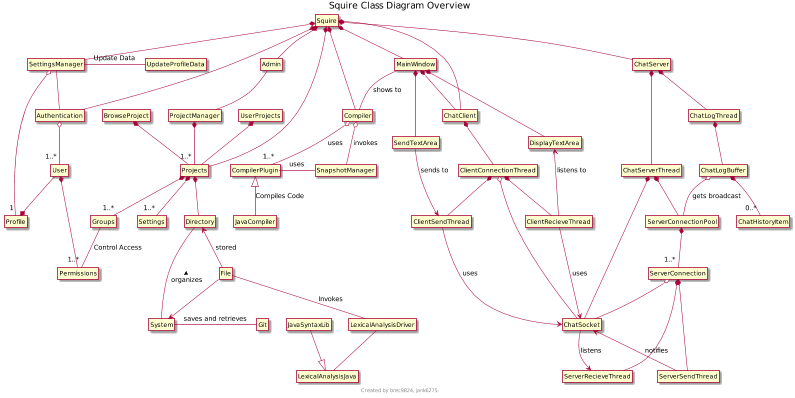
\includegraphics[width=1\textwidth]{diagrams/class-overview}
        \end{center}
        \captionof{figure}{Class overview of Squire displaying the connections between each subsystem and their classes.}
        %\captionof{figure}{Each team should assign one additional "overview" subteam to draw one or more higher-level overview class diagrams showing the aggregated big picture, with more classes and associations showing but less class detail. This could be one giant diagram, or separate diagrams for inheritance, aggregation, and user-defined associations, or provide an overview along some other structured lines.}
    \end{minipage}

\section{Authentication (mora5651)}
    \begin{minipage}{1\textwidth}
        \begin{center}
            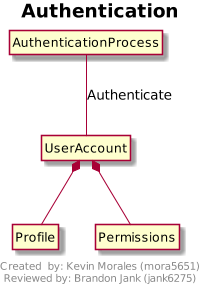
\includegraphics[width=0.5\textwidth]{diagrams/class-authentication}
        \end{center}
        \captionof{figure}{Authentication is a security precaution in sQuire that allows the system to verify a user. Users will provide a username and password, and will be validated on the server-side. Sequence diagram for Authentication can be found at 6.1.}
    \end{minipage}

\section{Project Management (bolt1003) (Sequence Diagram 6.2)}
    \begin{minipage}{1\textwidth}
        \begin{center}
            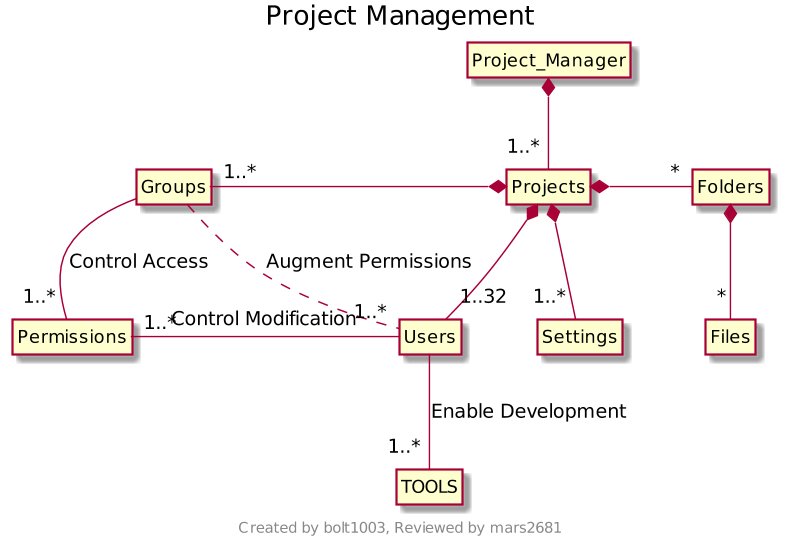
\includegraphics[width=0.9\textwidth]{diagrams/class-projectmanagement}
        \end{center}
        \captionof{figure}{Project management allows for the group to delicate permissions and create projects}
    \end{minipage}

\section{Project Ideas (mars2681)}
    \begin{minipage}{1\textwidth}
        \begin{center}
            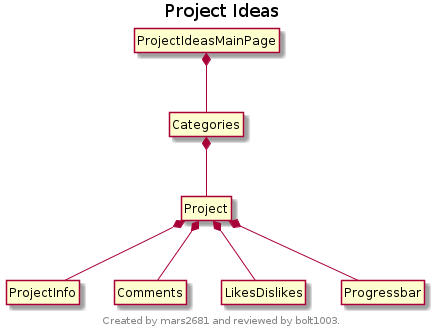
\includegraphics[width=0.7\textwidth]{diagrams/class-ProjectIdeas}
        \end{center}
        \captionof{figure}{The Project Ideas page allows the user to browse other user's projects ideas, as well as create and customize their own project ideas. It starts at the main page. From here, the user can select to view their own projects, and from there create, delete, or edit their ideas. Also at the main page, users can view other projects. Here will be categories of projects, the most popular projects, and new projects. Through browsing these pages, the user can see the description of projects, the amount of support, likes, dislikes, and they can follow and pledge their assistance to the project.}
    \end{minipage}

\section{Settings, Preferences, and Profile (brec9824)}
    \begin{minipage}{1\textwidth}
        \begin{center}
            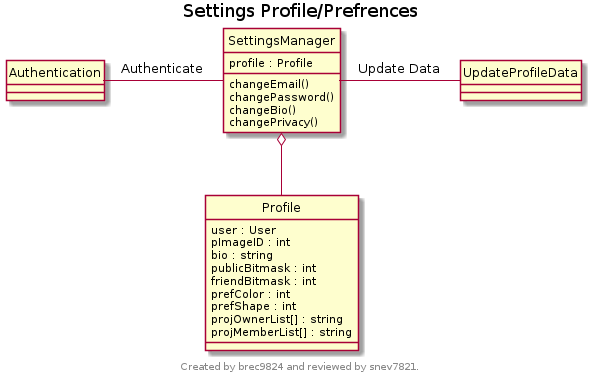
\includegraphics[width=0.9\textwidth]{diagrams/class-SettingsManager}
        \end{center}
        \captionof{figure}{Settings Profile/Prefrences allows for profile viewing and management while maintaining speed with the use of push updates. SettingsManager uses Authentication to verify valid input and to authentic the users data. While SettingsManager uses UpdateUserProfile to push the users data that needs to updated to the server. Sequence Diagram for a settings change can be found at 6.4}
    \end{minipage}

\section{Compiler (boss2849) (Sequence Diagram 6.5)}
    \begin{minipage}{1\textwidth}
        \begin{center}
            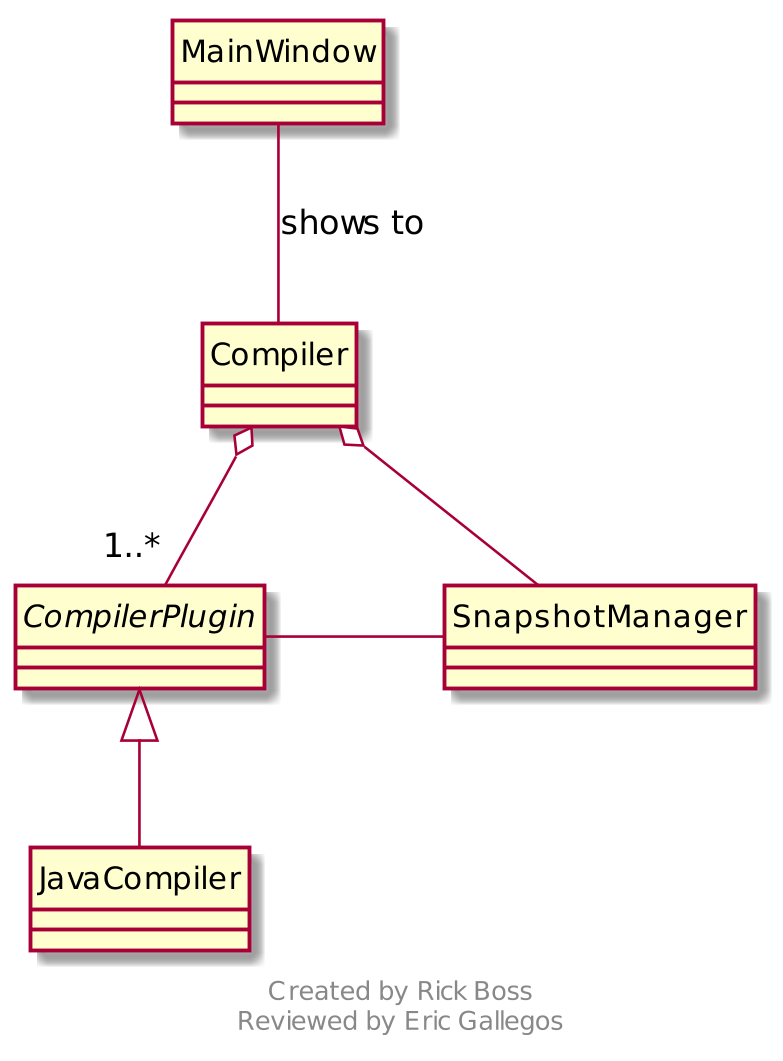
\includegraphics[width=0.7\textwidth]{diagrams/class-compiler}
        \end{center}
        \captionof{figure}{The Compiler is invoked from the main window. From here, the Compiler will select the appropriate CompilerPlugin determined by the configured compiler for the project. The compiler also invokes the SnapshotManager, which stores the current state of the code to be used during compilation. In this simple example, only a JavaCompiler plugin is present, but there can be more than one plugins available in the future. The JavaCompiler plugin retrieves the code snapshot from the SnapshotManager and compiles the code.}
    \end{minipage}

\section{Syntax (gall7417)}
    \begin{minipage}{1\textwidth}
        \begin{center}
            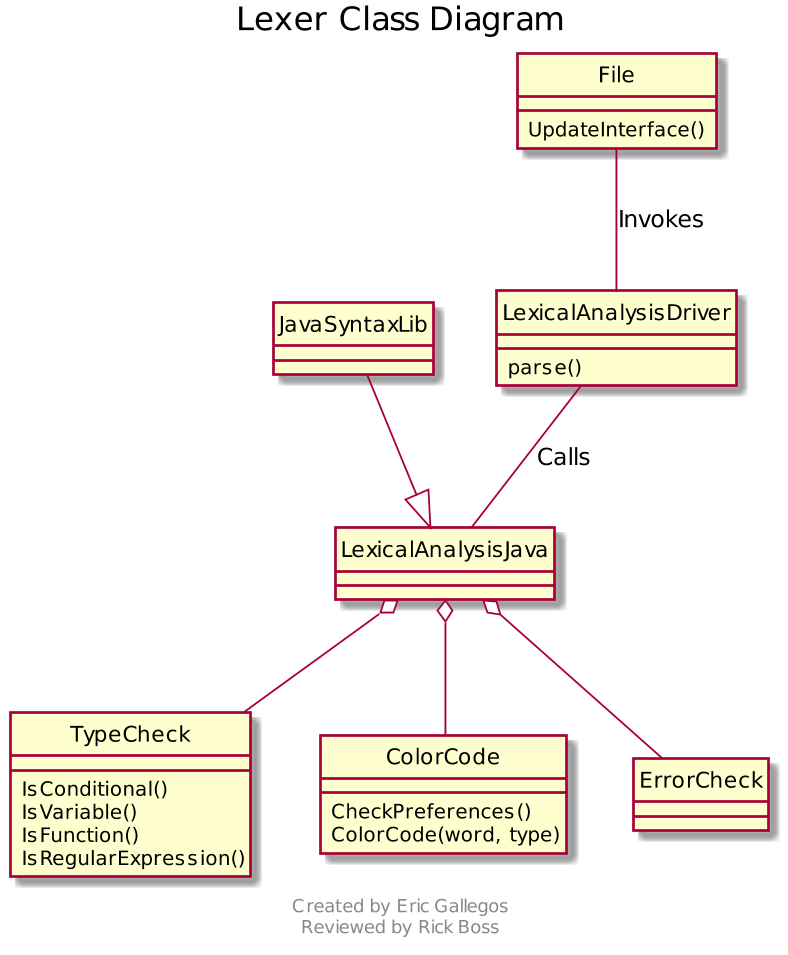
\includegraphics[width=0.9\textwidth]{diagrams/class-lexer}
        \end{center}
        \captionof{figure}{The File class regularly invokes the Lexical Analysis class to give feedback to users code input. The Lexical Analysis driver calls the corresponding Lexical Analysis class for the language used (Java). This language specific class checks for errors using the ErrorCheck class, searches for word types using the TypeCheck class, and will assign the various words colors to reflect the word types using the ColorCode class.}
    \end{minipage}

\section{Communication (jank6275)}
    \begin{minipage}{1\textwidth}
        \begin{center}
            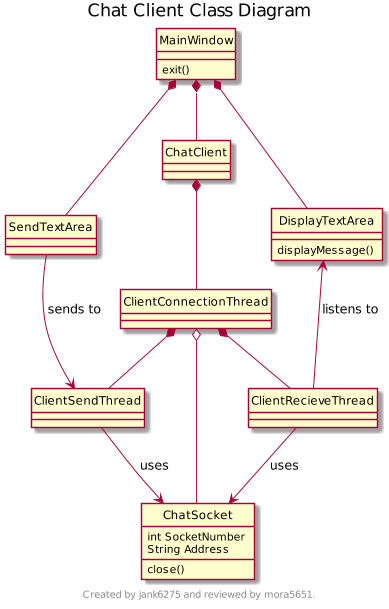
\includegraphics[width=0.7\textwidth]{diagrams/class-communication-client}
        \end{center}
        \captionof{figure}{The ChatClient class will handle text communication in conjuction with the ChatServer class. The Main Window will be home to the ChatClient. The ChatClinet will consist of client send/recieve threads to handle user input/output in the Main Window via the ChatSocket.}
    \end{minipage}
    \newpage
    \begin{minipage}{1\textwidth}
        \begin{center}
            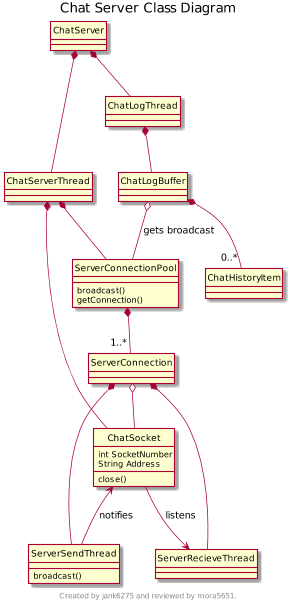
\includegraphics[width=0.5\textwidth]{diagrams/class-communication-server}
        \end{center}
        \captionof{figure}{The ChatServer class will handle text communication between ChatClient(s). The ChatLogThead records any messages broadcast by chat clients in the ServerConnectionPool as a ChatHistoryItem. Each ServerConnection consists of a send and recieve thread that utilize the ChatSocket to broadcast messages.}
    \end{minipage}

\section{Project File Editor (snev7821)}
    \begin{minipage}{1\textwidth}
        \begin{center}
            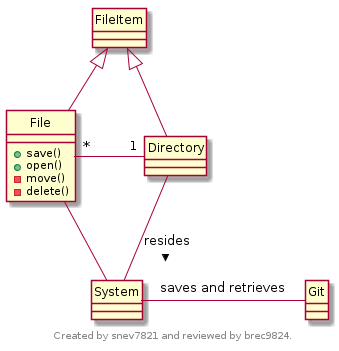
\includegraphics[width=0.7\textwidth]{diagrams/class-ProjectFileEditor}
        \end{center}
        \captionof{figure}{The project File Editor is simply the file system for Squire. It provides basic read/write permission for any user related to a project. Only admins of a project may move project files, delete old files, and create new files.}
    \end{minipage}
    %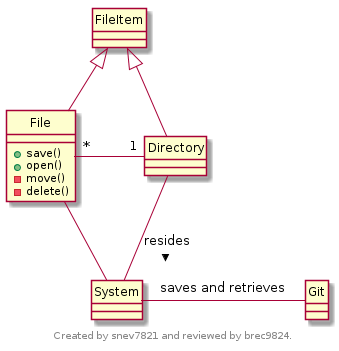
\includegraphics[scale=0.7]{diagrams/ProjectFileEditor-snev7821}
    %The project File Editor is simply the file system for Squire. It provides basic read/write permission for any user related to a project. Only admins of a project may move %project files, delete old files, and create new files.

%##########################################################################################################################################################################
% Sequence Diagrams
%##########################################################################################################################################################################

\chapter{Sequence Diagrams}
\section{Authentication (jank6275)}
    \subsection{Login}
        \begin{minipage}{1\textwidth}
            \begin{center}
                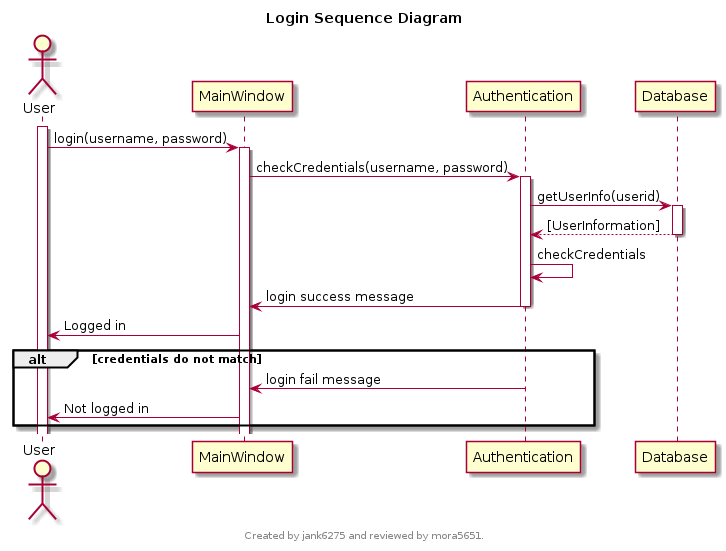
\includegraphics[width=0.7\textwidth]{diagrams/sequence-authentication-login}
            \end{center}
            \captionof{figure}{A sequence diagram for logging in to Squire.}
        \end{minipage}
    \subsection{Logout}
        \begin{minipage}{1\textwidth}
            \begin{center}
                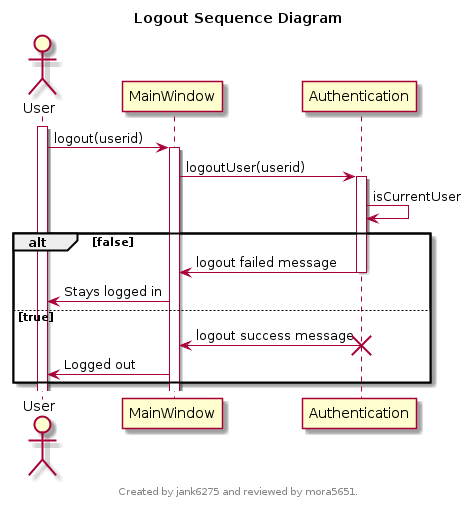
\includegraphics[width=0.7\textwidth]{diagrams/sequence-authentication-logout}
            \end{center}
            \captionof{figure}{A sequence diagram for logging out of Squire.}
        \end{minipage}
    \subsection{Register}
        \begin{minipage}{1\textwidth}
            \begin{center}
                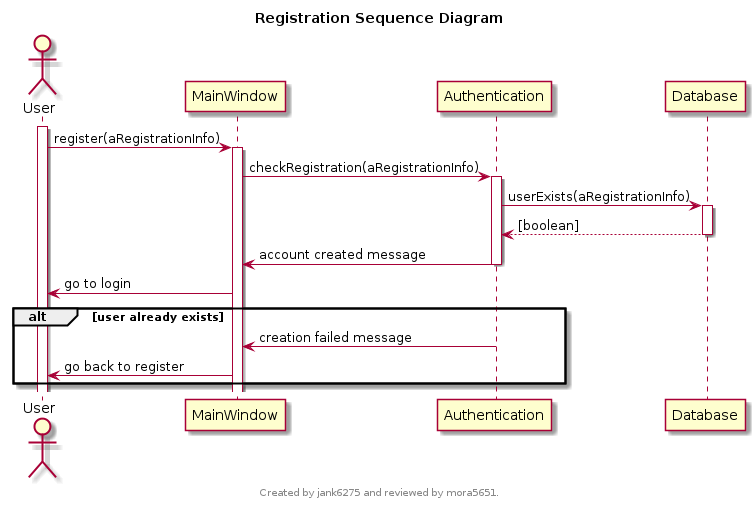
\includegraphics[width=0.7\textwidth]{diagrams/sequence-authentication-register}
            \end{center}
            \captionof{figure}{A sequence diagram for registering a nmew account with Squire.}
        \end{minipage}
    
\section{Project Management (mars2681)}
    \begin{minipage}{1\textwidth}
        \begin{center}
            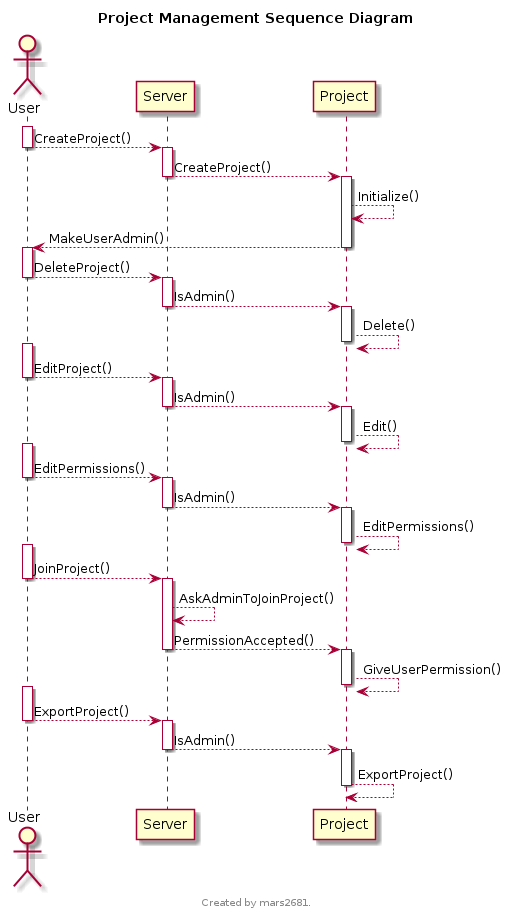
\includegraphics[width=0.7\textwidth]{diagrams/sequence-projectmanagement}
        \end{center}
        \captionof{figure}{A sequence diagram showing how user can manage their projects}
    \end{minipage}
    
\section{Project Ideas (snev7821)}
    \begin{minipage}{1\textwidth}
        \begin{center}
            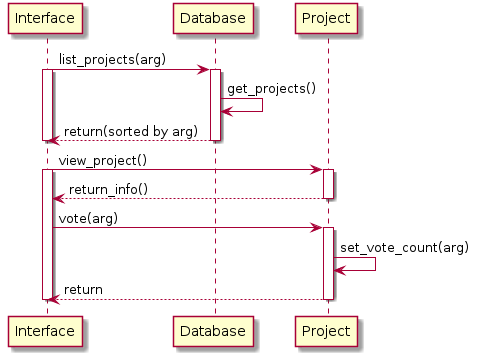
\includegraphics[width=0.7\textwidth]{diagrams/sequence-projectideas}
        \end{center}
        %\captionof{figure}{The section where the user browses projects and can up or downvote other projects. Args for list_project are how the user would like to sort the project.}
    \end{minipage}
    
\section{Settings, Preferences, and Profile (gall7417)}
    \begin{minipage}{1\textwidth}
        \begin{center}
            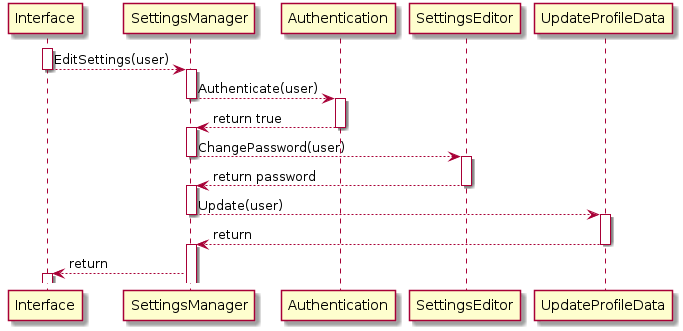
\includegraphics[width=0.7\textwidth]{diagrams/SettingsSequenceDiagram}
        \end{center}
        \captionof{figure}{Example of a sequence during a users profile settings change. In this case the user is changing his password, however a similar sequence would apply for other profile settings.}
    \end{minipage}
    
\section{Compiler (bolt1003)}
    \begin{minipage}{1\textwidth}
        \begin{center}
            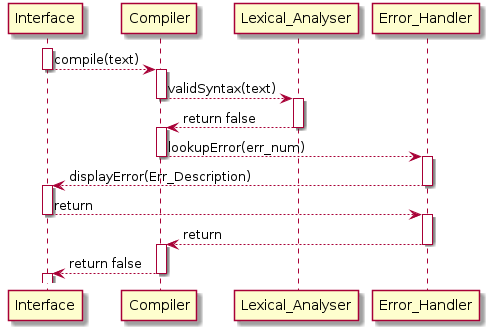
\includegraphics[width=0.7\textwidth]{diagrams/sequence-compiler}
        \end{center}
        \captionof{figure}{The sequence of a user attempting to compile a program with a syntax error.}
    \end{minipage}
    
\section{Syntax (mora5651)}
    \begin{minipage}{1\textwidth}
        \begin{center}
            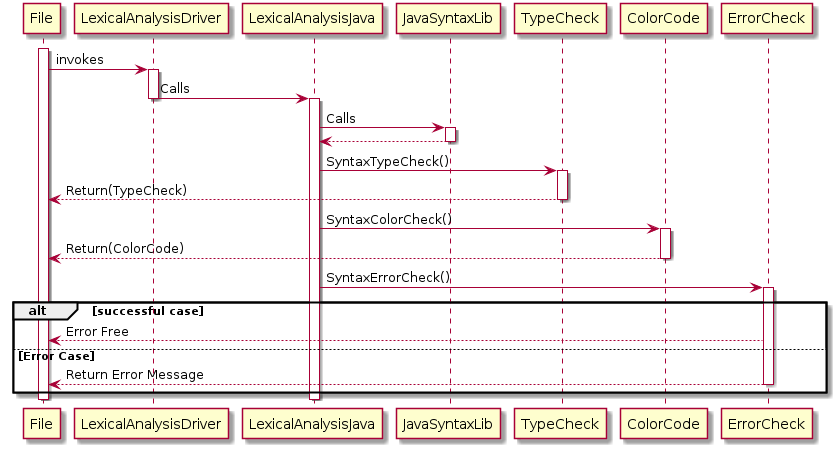
\includegraphics[width=0.7\textwidth]{diagrams/sequence-syntax}
        \end{center}
        \captionof{figure}{Sequence diagram for java syntax in the file editor being updated in real-time.}
    \end{minipage}
    
\section{Communication (boss2849)}
    \begin{minipage}{1\textwidth}
        \begin{center}
            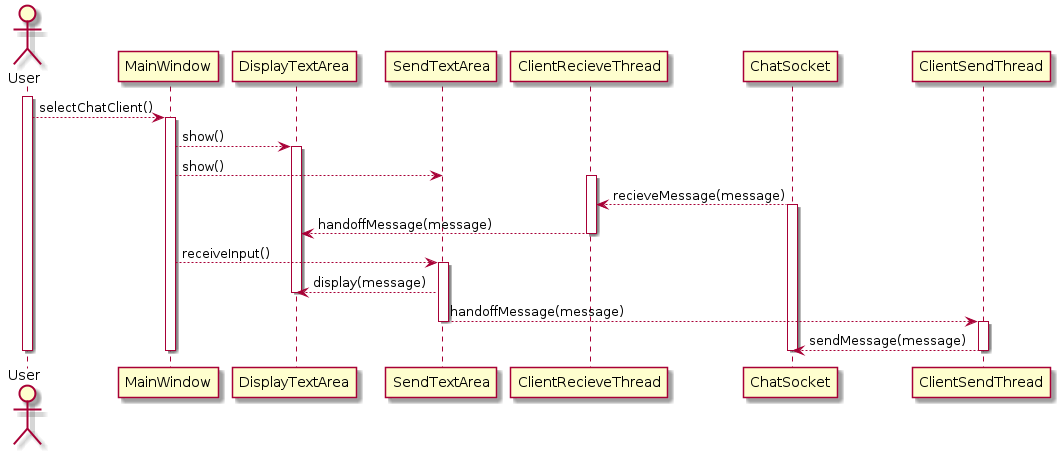
\includegraphics[width=1.0\textwidth]{diagrams/sequence-chat-client}
        \end{center}
        \captionof{figure}{Sequence diagram for chat client interaction.}
        \begin{center}
            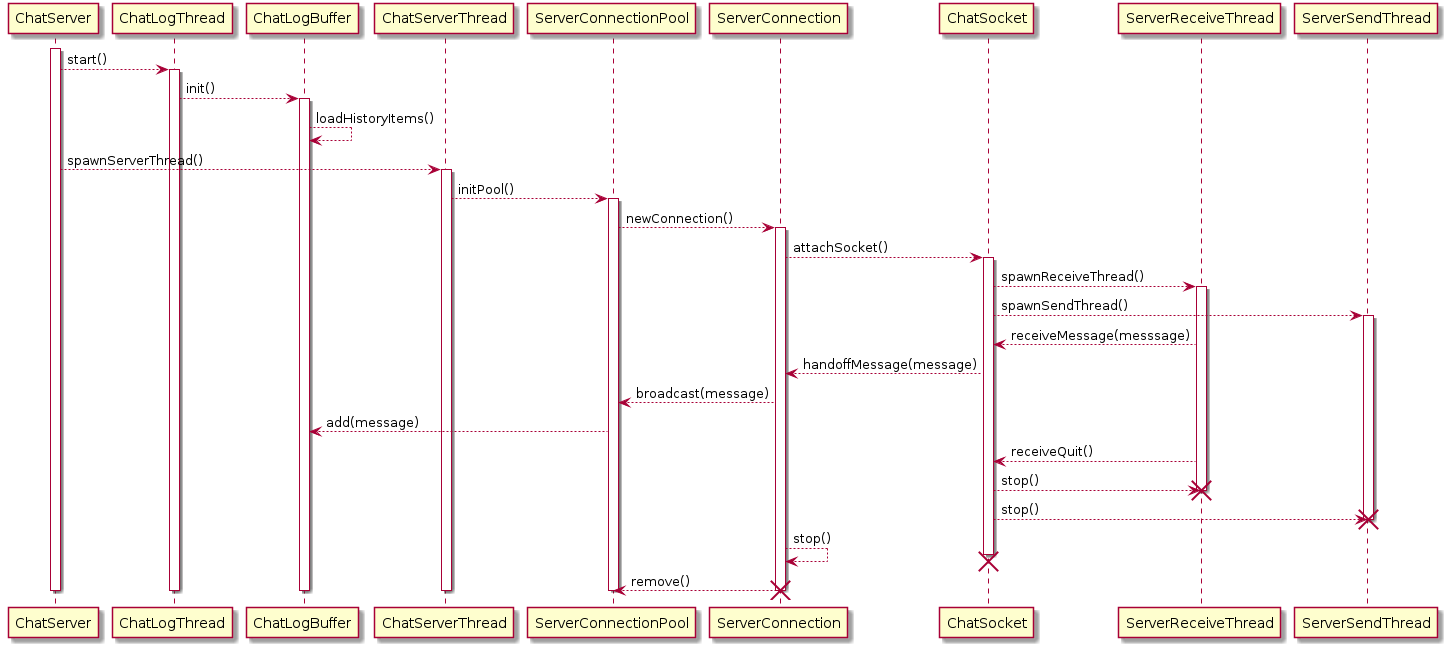
\includegraphics[width=1.0\textwidth]{diagrams/sequence-chat-server}
        \end{center}
        \captionof{figure}{Sequence diagram for chat server interaction.}
    \end{minipage}
    
\section{Project File Editor (brec9824)}
    \begin{minipage}{1\textwidth}
        \begin{center}
            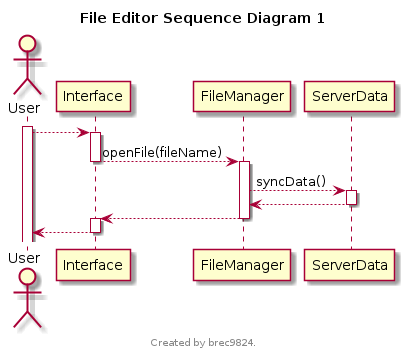
\includegraphics[width=0.7\textwidth]{diagrams/sequence-projectfileeditor1}
        \end{center}
        \captionof{figure}{Sequence diagram showing the control structure of opening a file in the project file editor. This sequence also relates to delete file, import file and add file.}
        \begin{center}
            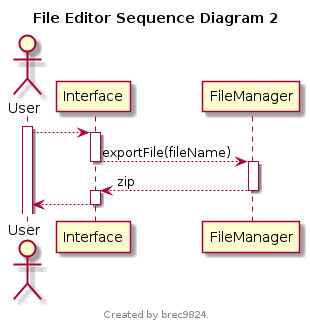
\includegraphics[width=0.7\textwidth]{diagrams/sequence-projectfileeditor2}
        \end{center}
        \captionof{figure}{Sequence diagram showing the control structure of exporting a file in the project file editor.}
    \end{minipage}
    
%##########################################################################################################################################################################
% Statecharts
%##########################################################################################################################################################################
\chapter{Statecharts}

    \section{Project Forum (snev7821)}
        \begin{minipage}{1\textwidth}
            \begin{center}
                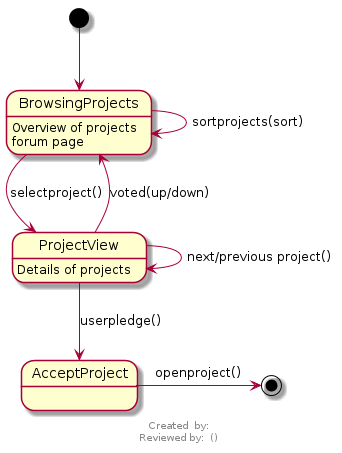
\includegraphics[width=0.5\textwidth]{diagrams/statechart-projectforum}
            \end{center}
            \captionof{figure}{Statechart showing the flow of a user browsing the project forum page}
        \end{minipage}
    
    \section{Settings/Preferences (gall7417)}
        \begin{minipage}{1\textwidth}
            \begin{center}
                %Missing statechart----------------> 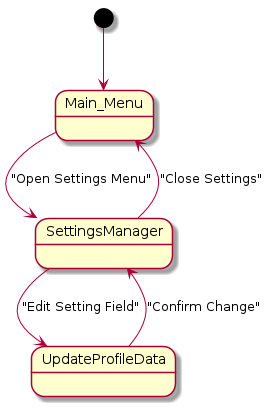
\includegraphics[width=0.5\textwidth]{diagrams/SettingsStateDiagram}
            \end{center}
            \captionof{figure}{Statechart showing the flow of a user changing a user setting}
        \end{minipage}

    \section{Compile (boss2849)}
        \begin{minipage}{1\textwidth}
            \begin{center}
                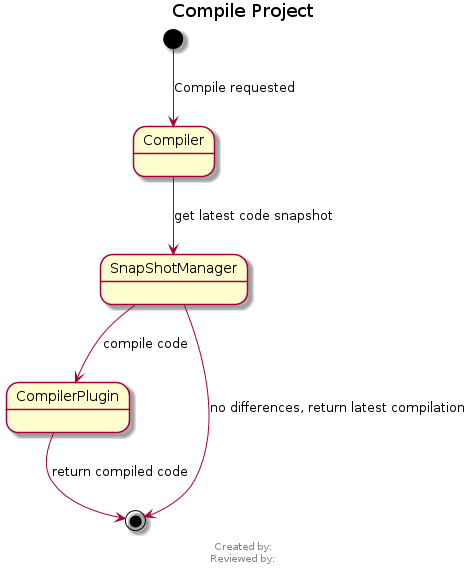
\includegraphics[width=0.5\textwidth]{diagrams/statechart-compile}
            \end{center}
            \captionof{figure}{Statechart showing the flow of a user compiling a file, or entire project.}
        \end{minipage}
        
    \section{Project Management (bolt1003)}
        \begin{minipage}{1\textwidth}
            \begin{center}
                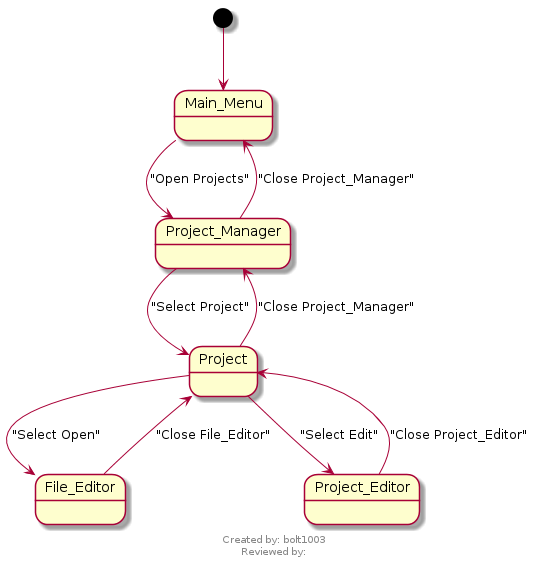
\includegraphics[width=0.5\textwidth]{diagrams/statechart-project_management}
            \end{center}
            \captionof{figure}{.}
        \end{minipage}
        
    \section{Communication (jank6275)}
        \begin{minipage}{1\textwidth}
            \begin{center}
                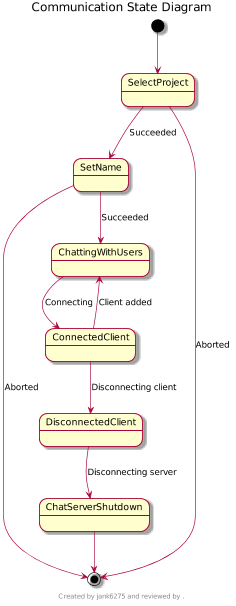
\includegraphics[width=0.5\textwidth]{diagrams/statechart-communication}
            \end{center}
            \captionof{figure}{A statechart that shows the various states of the communication system.}
        \end{minipage}
        
    \section{Authentication (brec9824)}
        \begin{minipage}{1\textwidth}
            \begin{center}
                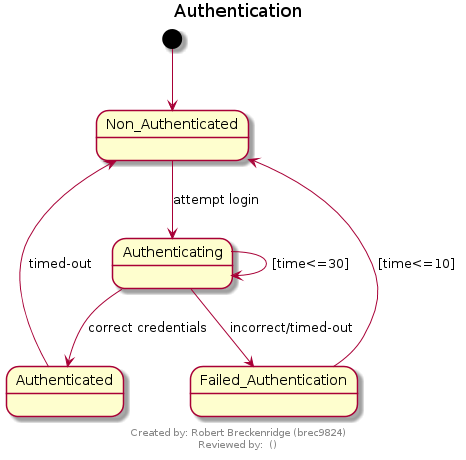
\includegraphics[width=0.5\textwidth]{diagrams/statechart-authentication-brec9824}
            \end{center}
            \captionof{figure}{Statechart showing the flow between states for authentication.}
        \end{minipage}

%##########################################################################################################################################################################
% Mockups
%##########################################################################################################################################################################

\chapter{Mockups}

    \section{Project Management (bolt1003)}
    \begin{minipage}{1\textwidth}
        \begin{center}
            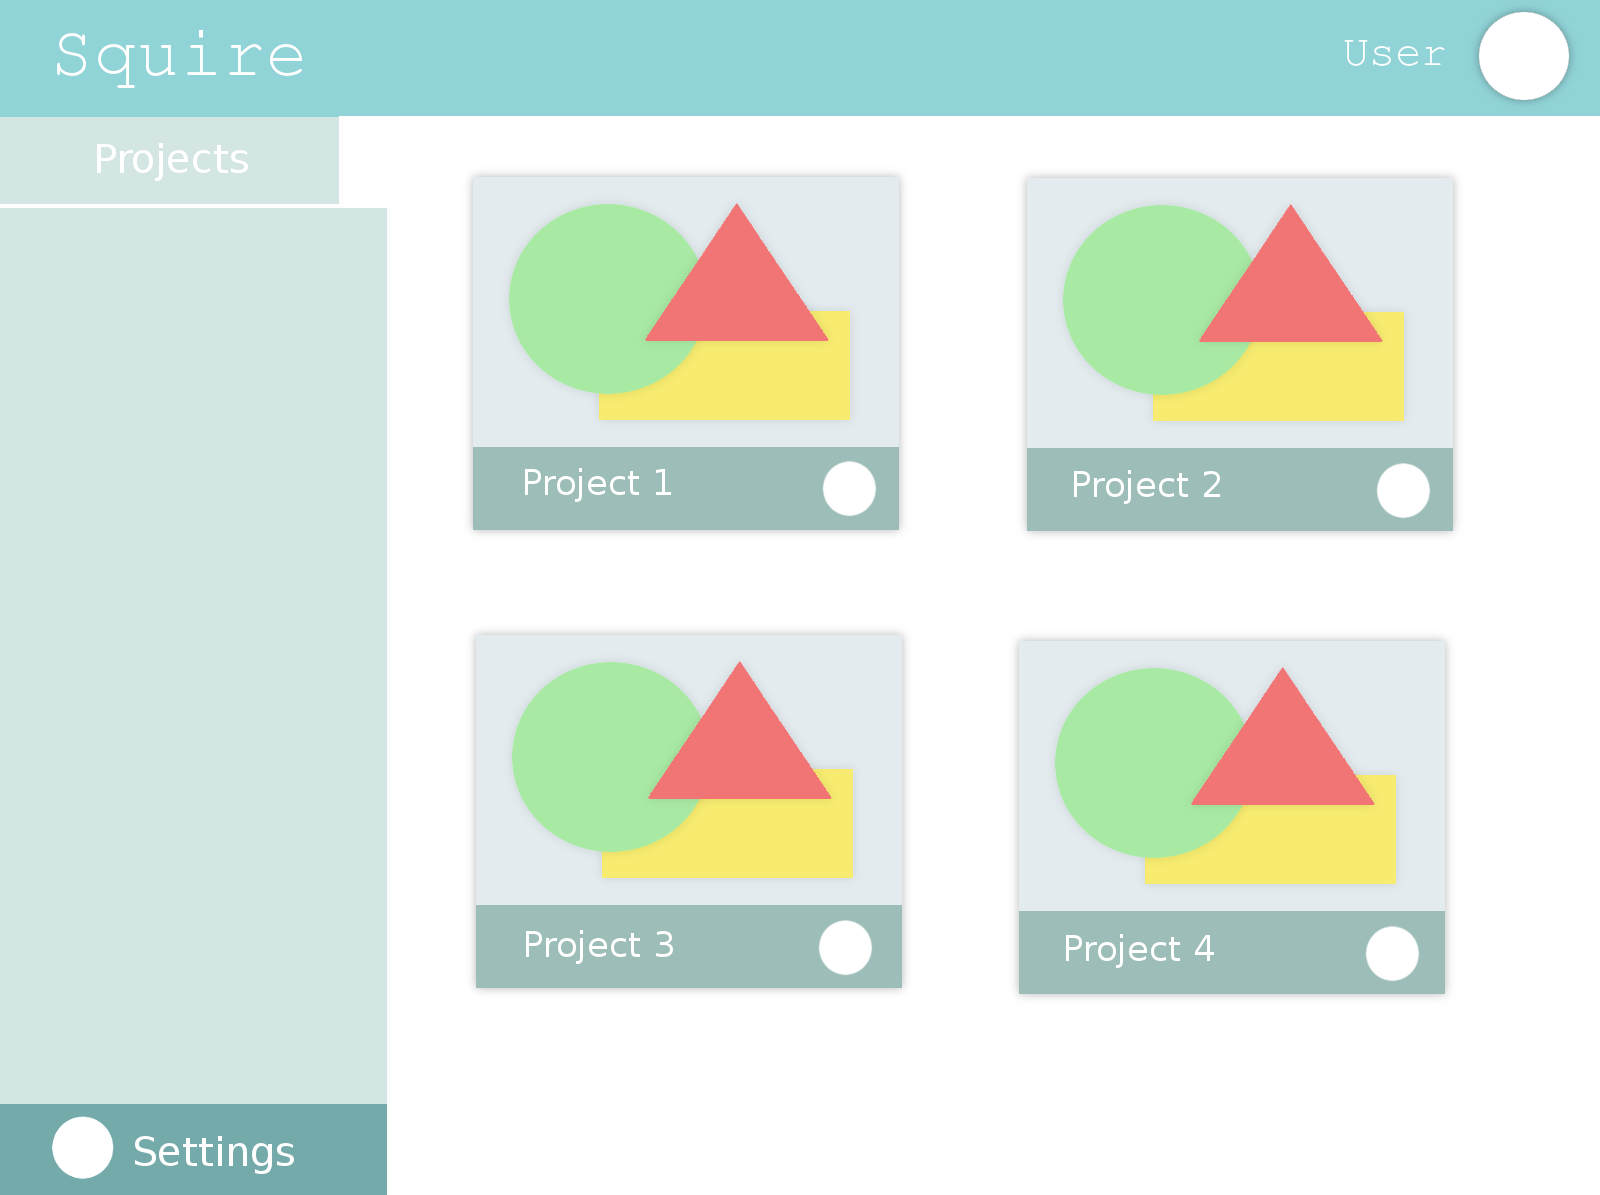
\includegraphics[width=0.9\textwidth]{mockups/mockup-project_management-bolt1003}
        \end{center}
        \captionof{figure}{A possible look for the project management page}
    \end{minipage}
    
    \section{Settings and Preferences (gall7417)}
    \begin{minipage}{1\textwidth}
        \begin{center}
            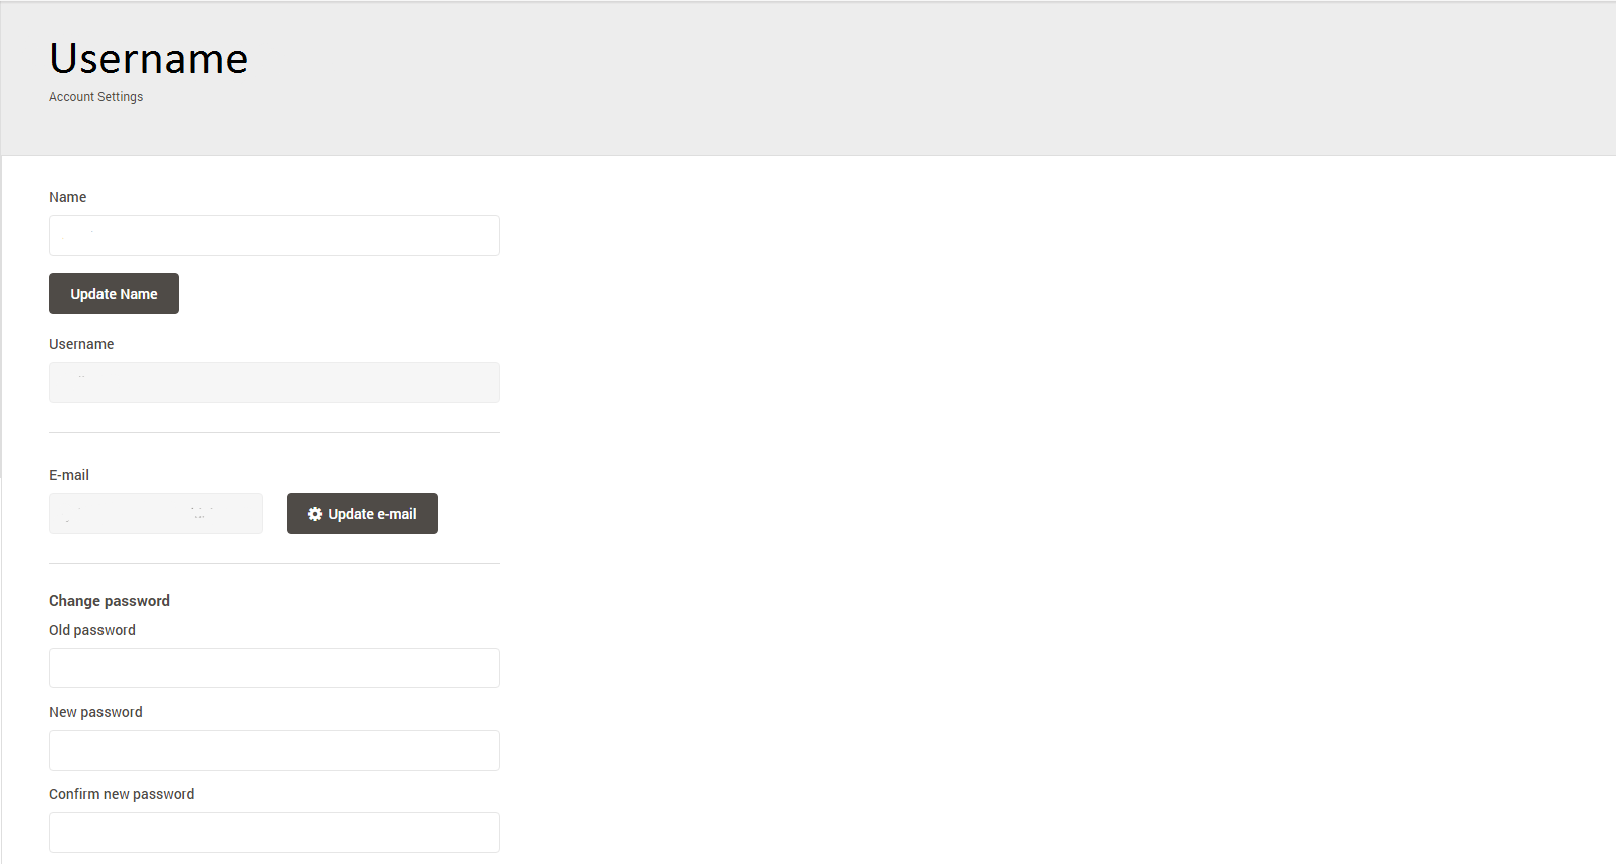
\includegraphics[width=0.9\textwidth]{mockups/mockup-settings-gall7417}
        \end{center}
        \captionof{figure}{Po}
    \end{minipage}
    
    \section{Squire Editor (jank6275)}
    \begin{minipage}{1\textwidth}
        \begin{center}
            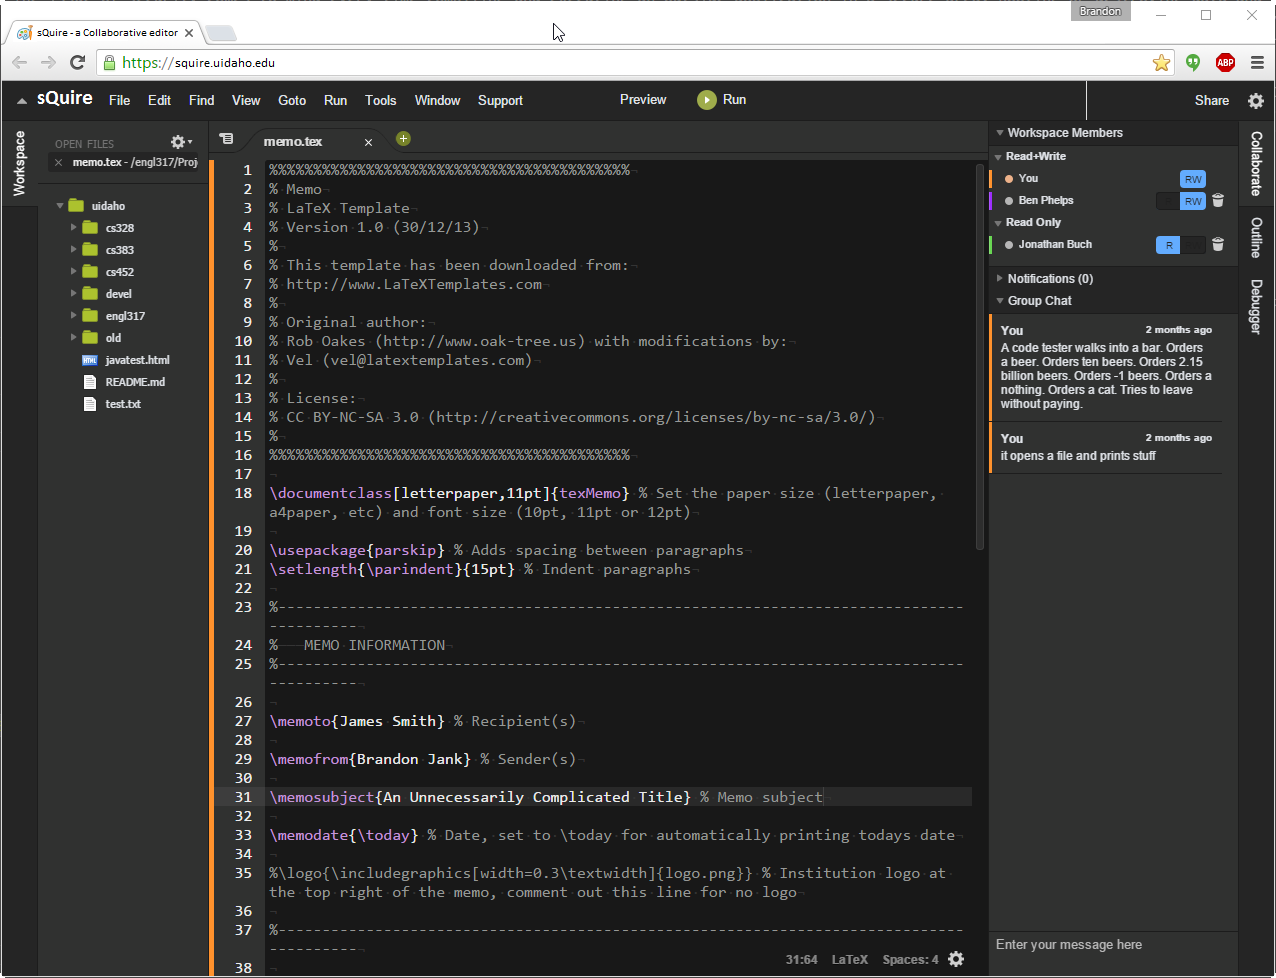
\includegraphics[width=0.9\textwidth]{mockups/mockup-editor-jank6275}
        \end{center}
        \captionof{figure}{What we envision Squire IDE to look like.}
    \end{minipage}
    
    \section{Squire Chat (jank6275)}
    \begin{minipage}{1\textwidth}
        \begin{center}
            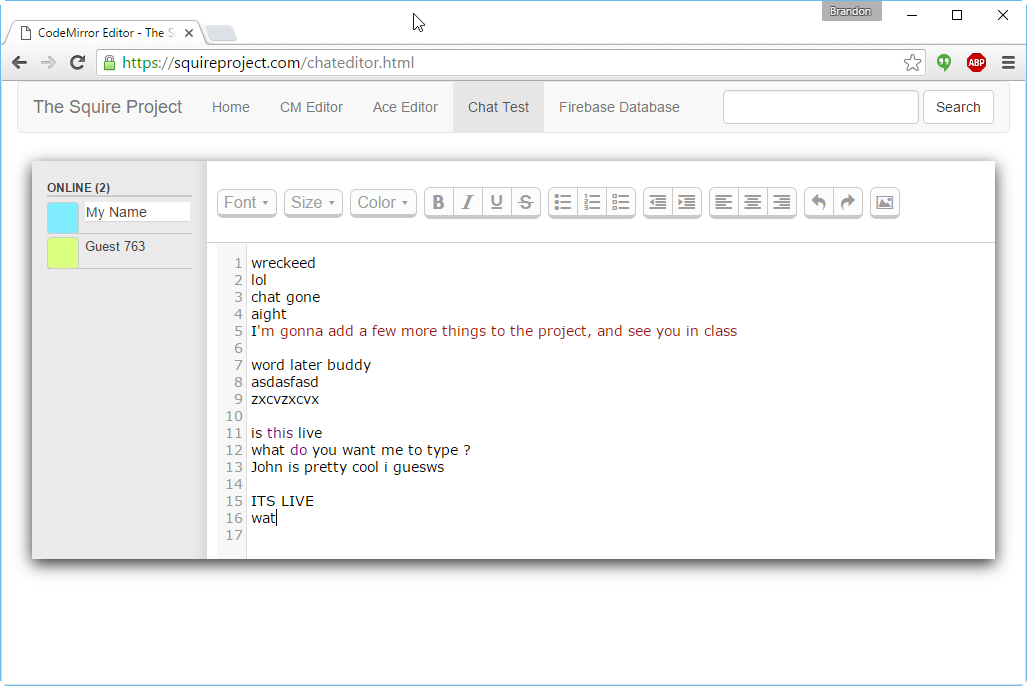
\includegraphics[width=0.9\textwidth]{mockups/mockup-communication-jank6275}
        \end{center}
        \captionof{figure}{How communication could work in squire.}
    \end{minipage}
    
    \section{Project Browser (snev7821)}
    \begin{minipage}{1\textwidth}
        \begin{center}
            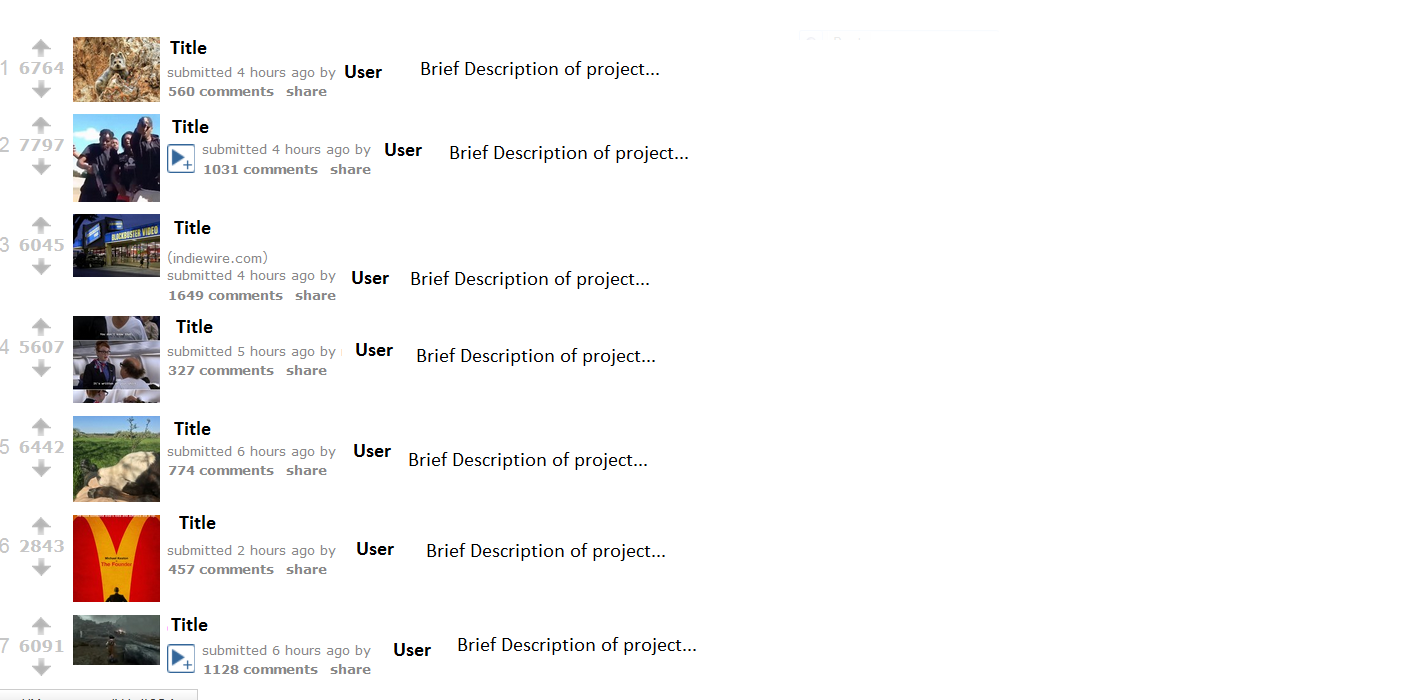
\includegraphics[width=0.9\textwidth]{mockups/mockup-project_browser-snev7821}
        \end{center}
        \captionof{figure}{Created from Paint and Reddit, the project browser may end up looking somewhat similar}
    \end{minipage}
    
    \section{Compile Mockup (boss2849)}
    \begin{minipage}{1\textwidth}
        \begin{center}
            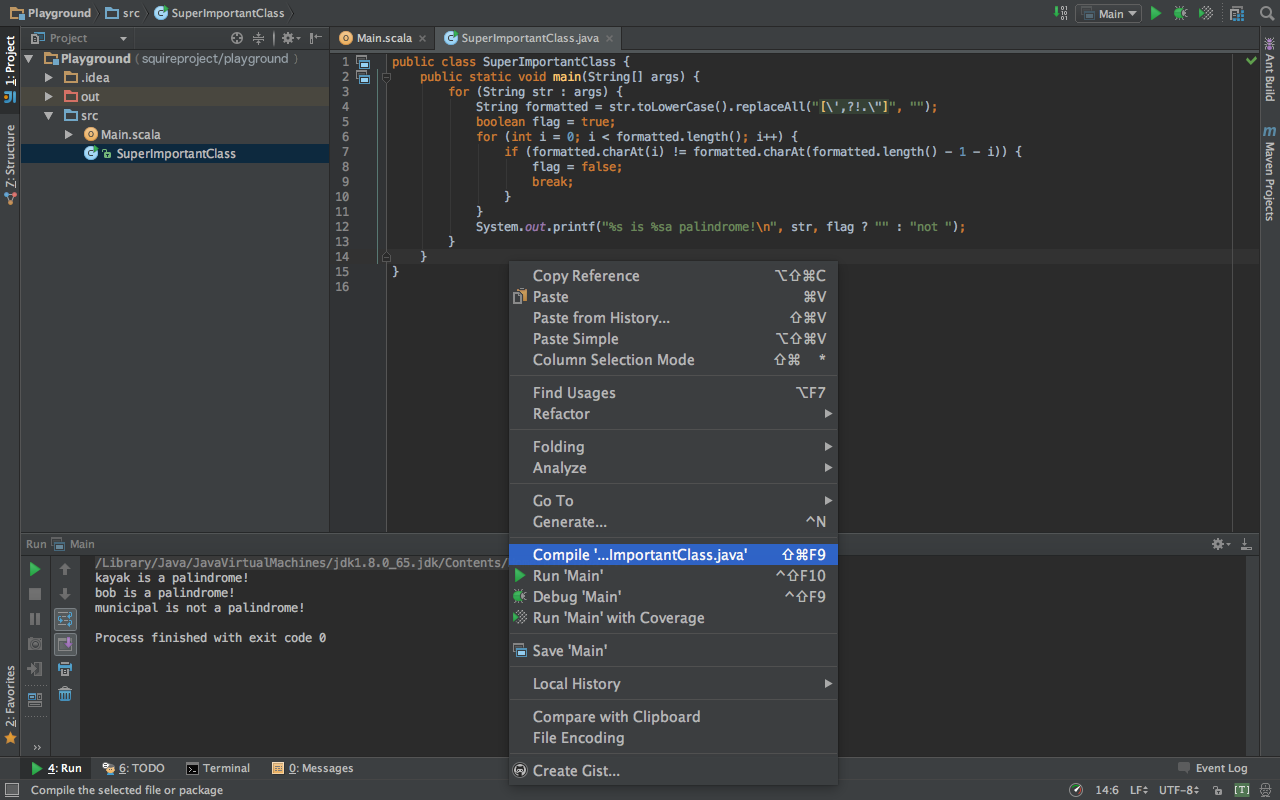
\includegraphics[width=0.9\textwidth]{mockups/mockup-compile-boss2849}
        \end{center}
        \captionof{figure}{A mockup, based off IntelliJ of compiling a file.}
    \end{minipage}

    \section{Syntax Mockup (mars2681)}
    \begin{minipage}{1\textwidth}
        \begin{center}
            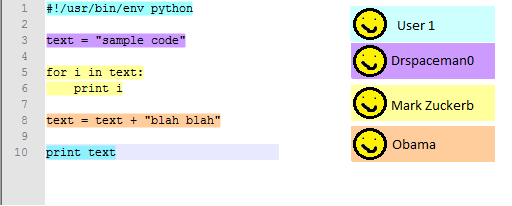
\includegraphics[width=0.9\textwidth]{mockups/mockup-syntax-mars2681}
        \end{center}
        \captionof{figure}{A mockup, created from Notepad++ and paint. Each user's input has its own shade. The light blue shade on Line 10 shows current user's cursor position.}
    \end{minipage}
    
    \section{Home (brec9824)}
    \begin{minipage}{1\textwidth}
        \begin{center}
            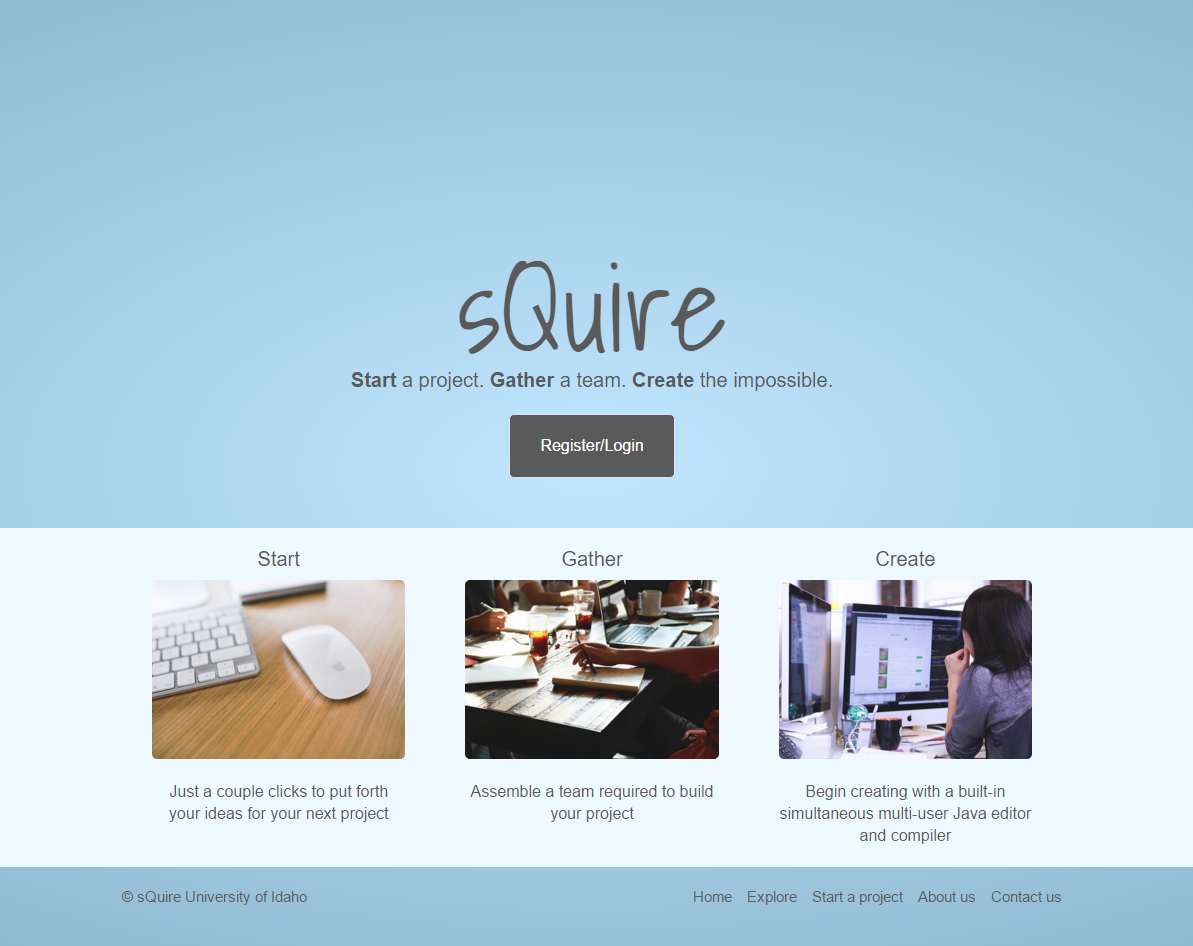
\includegraphics[width=0.9\textwidth]{mockups/mockup-home-brec9824}
        \end{center}
        \captionof{figure}{A mockup for the look of squire's home page. Created using html and css.}
    \end{minipage}
    
    \section{Register (brec9824)}
    \begin{minipage}{1\textwidth}
        \begin{center}
            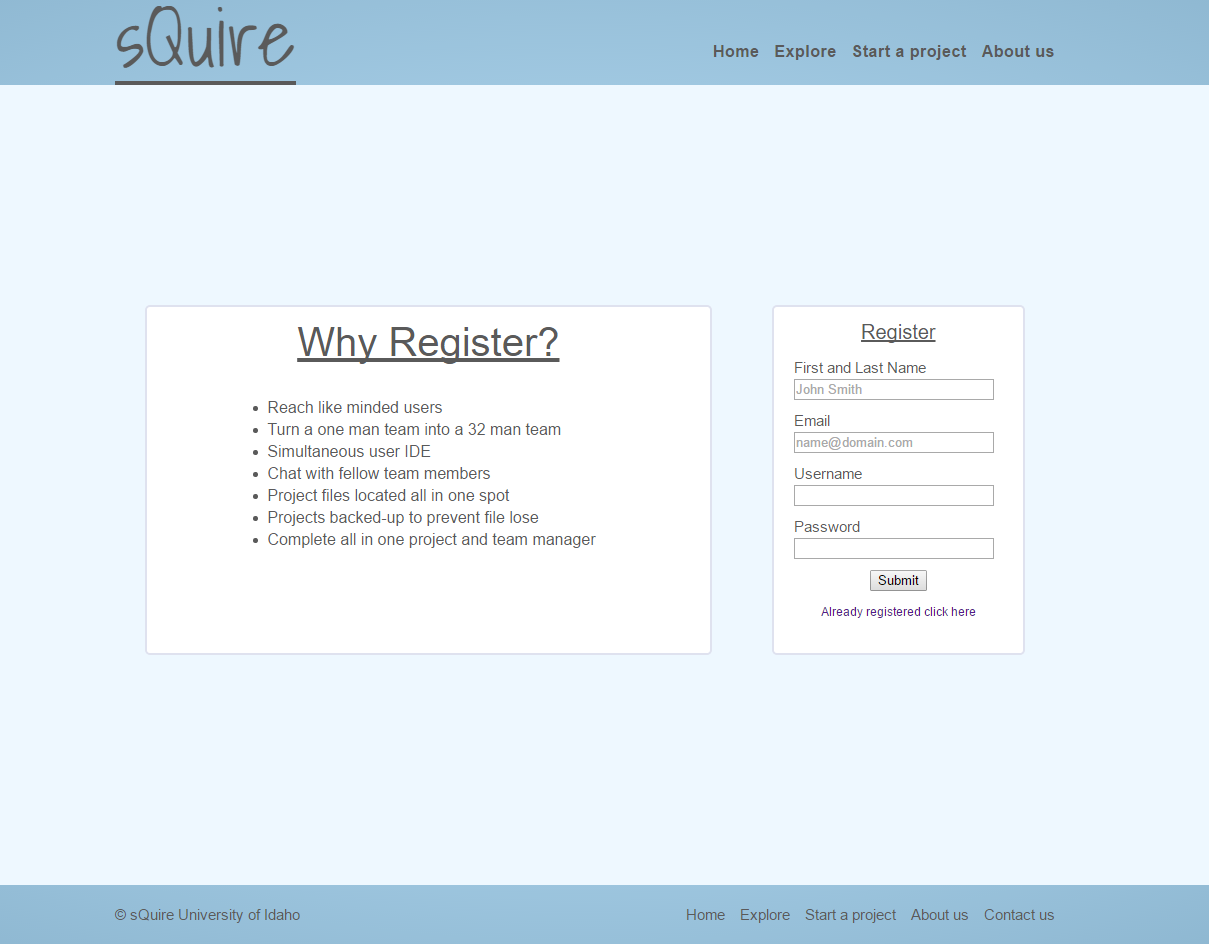
\includegraphics[width=0.9\textwidth]{mockups/mockup-register-brec9824}
        \end{center}
        \captionof{figure}{A mockup for the look of squire's register page. Created using html and css.}
    \end{minipage}
    
     \section{Login (brec9824)}
    \begin{minipage}{1\textwidth}
        \begin{center}
            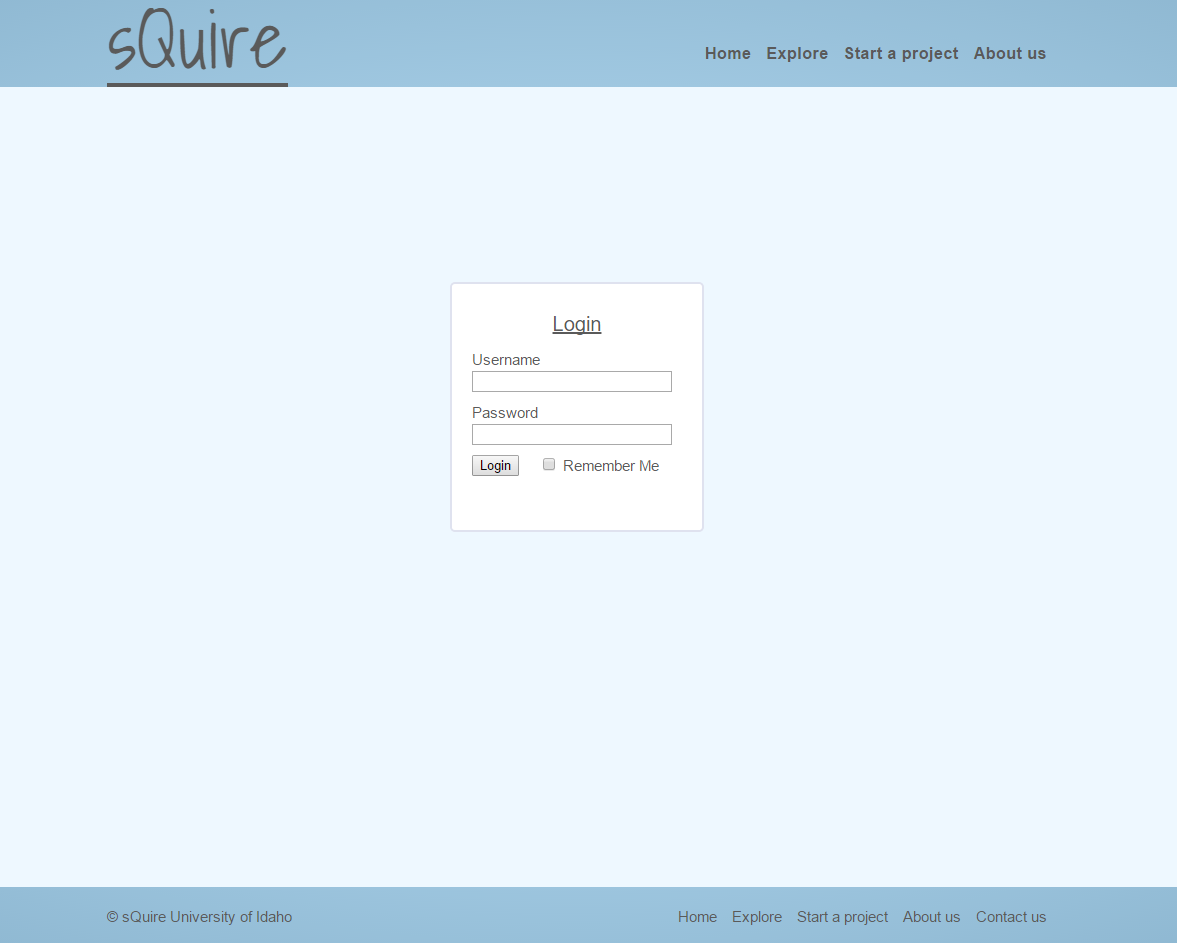
\includegraphics[width=0.9\textwidth]{mockups/mockup-login-brec9824}
        \end{center}
        \captionof{figure}{A mockup for the look of squire's login page. Created using html and css.}
    \end{minipage}
    
    \section{Project Finder (brec9824)}
    \begin{minipage}{1\textwidth}
        \begin{center}
            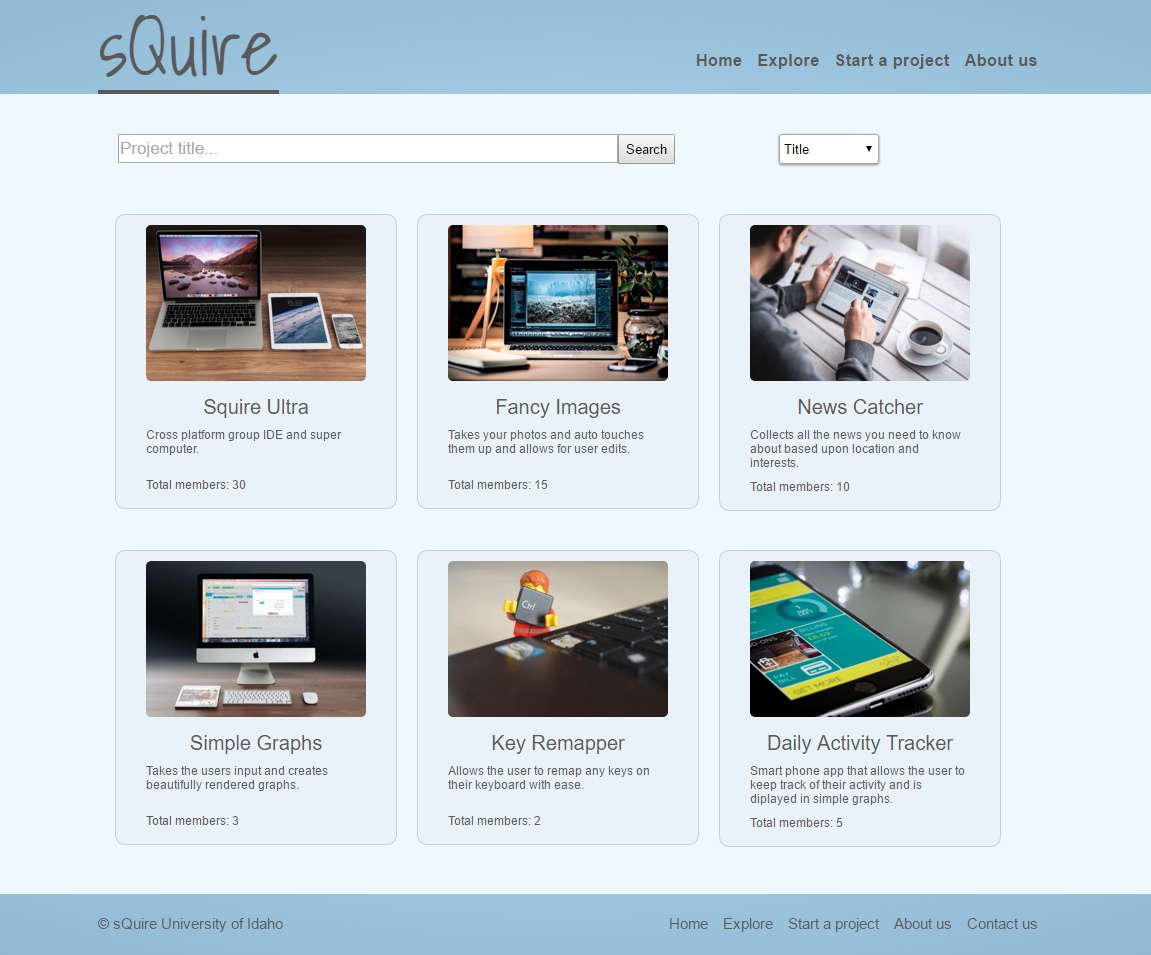
\includegraphics[width=0.9\textwidth]{mockups/mockup-projectfinder-brec9824}
        \end{center}
        \captionof{figure}{A mockup for the look of squire's project finder page. Created using html and css.}
    \end{minipage}
    
    \section{Project Idea (mora5651)}
    \begin{minipage}{1\textwidth}
        \begin{center}
            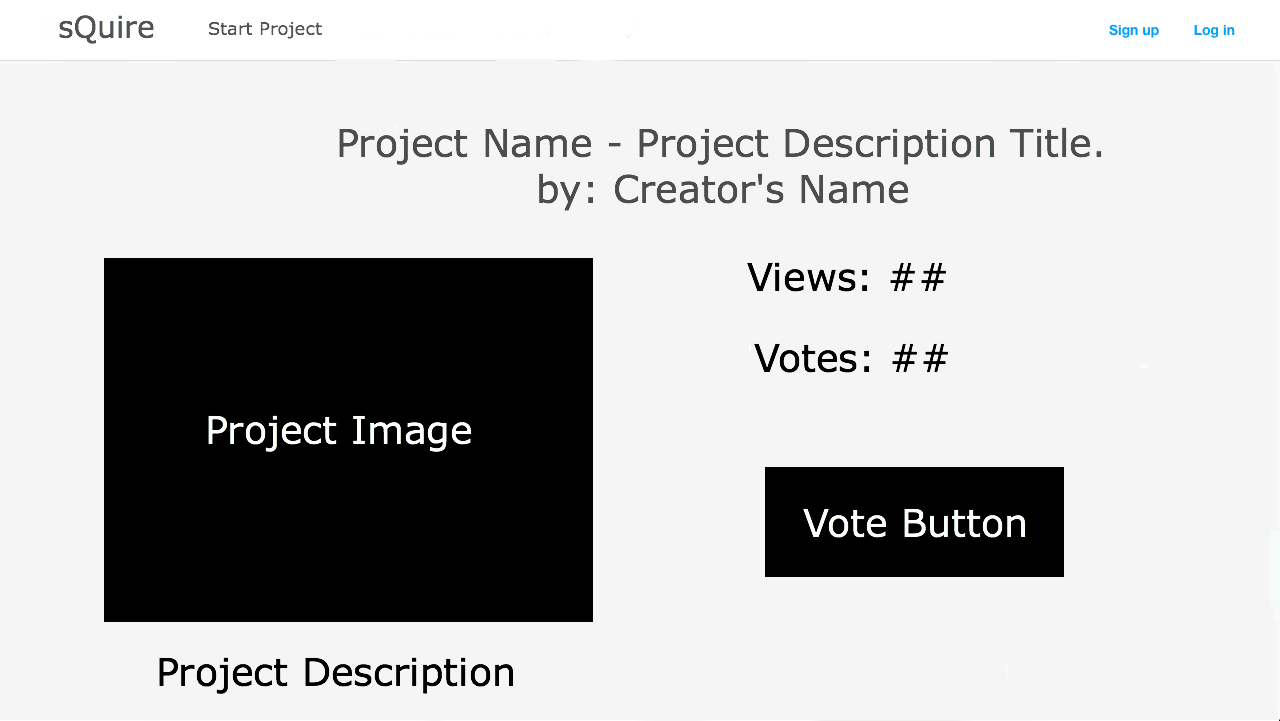
\includegraphics[width=0.9\textwidth]{mockups/mockup-ProjectIdea-mora5651}
        \end{center}
        \captionof{figure}{A mockup of how the project idea page should look like.}
    \end{minipage}
    
%##########################################################################################################################################################################
% Implimentations
%##########################################################################################################################################################################

\chapter{Implementation}
    \section{Overview}
    \begin{minipage}{1\textwidth}
        \begin{center}
            \includegraphics[width=0.9\textwidth]{diagrams/folders-overview-max}
        \end{center}
        \captionof{figure}{Squire's file structure is organized to allow for a simple and concise project flow. This structure includes seven main subfolders app, bootstrap, config, database, public, resources, and tests. Each containing crucial files allowing squireproject.com to exist.}
    \end{minipage}
    \begin{itemize}
        \item Main Subfolders:
        \begin{itemize}
            \item app: Contains the files that allow for the main functionality of Squire
            \begin{itemize}
                \item Console: Artisan commands for Laravel’s built in commands.
                \item Events: Event classes for alerting different sub-systems to given actions.
                \item Exceptions: Exception handlers for dealing with exceptions.
                \item Http: Controllers for routing data to and from squireproject.com. Middleware usable by different aspects like authentication. Requests
                \item Jobs: Queue able jobs for Squire’s request cycle.
                \item Listeners: Handler classes for events to allow for performing actions based on triggered events.
                \item Policies: Authorization policy classes for dealing with user action.
                \item Providers: Addable 3rd-party features for extending built in features.
            \end{itemize}
            \item bootstrap: Contains files for configuring auto loading and for bootstrapping the framework.
            \item config: Contains project squires configuration files.
            \item database: Contains files pertaining to database migrations and seeds.
            \item public: Contains the front controller and web page assets.
            \begin{itemize}
                \item css: CSS files for html styling.
                \item images: Image files.
                \item js: Java scripts.
            \end{itemize}
            \item resources: Contains raw assets, front end views, and localization files.
            \begin{itemize}
                \item assests: raw assets like SASS.
                \item lang: setting messages and their languages used for user messages.
                \item views: front end html pages users see when viewing squireproject.com.
            \end{itemize}
            \item tests: tests: Contains files for automated testing.
        \end{itemize}
    \end{itemize}
    
    \section{Prototype Implementations}
        \subsection{Server Stack (jank6275)}
        \begin{minipage}{1\textwidth}
            \begin{center}
            \includegraphics[width=0.9\textwidth]{protos/proto-serverstack-jank6275}
            \end{center}
            \captionof{figure}{The internet domain squireproject.com was registered and an SSL certificate was generated for secure communications. A virtual private server was provisioned and Ubuntu 14.04 installed and then hardened to common network attack vectors. Nginx and MySQL were installed and configured. The web content was written in HTML and bootstrap CSS.}
        \end{minipage}
    
    

\end{document}